\documentclass{article} % For LaTeX2e
\usepackage{iclr2019_conference,times}
\usepackage{graphicx} % more modern
\usepackage{subfigure}
\usepackage{hhline}
\usepackage{comment}
\usepackage{amsmath}
\usepackage{wrapfig}
% Optional math commands from https://github.com/goodfeli/dlbook_notation.
%%%%% NEW MATH DEFINITIONS %%%%%

\usepackage{amsmath,amsfonts,bm}

% Mark sections of captions for referring to divisions of figures
\newcommand{\figleft}{{\em (Left)}}
\newcommand{\figcenter}{{\em (Center)}}
\newcommand{\figright}{{\em (Right)}}
\newcommand{\figtop}{{\em (Top)}}
\newcommand{\figbottom}{{\em (Bottom)}}
\newcommand{\captiona}{{\em (a)}}
\newcommand{\captionb}{{\em (b)}}
\newcommand{\captionc}{{\em (c)}}
\newcommand{\captiond}{{\em (d)}}

% Highlight a newly defined term
\newcommand{\newterm}[1]{{\bf #1}}


% Figure reference, lower-case.
\def\figref#1{figure~\ref{#1}}
% Figure reference, capital. For start of sentence
\def\Figref#1{Figure~\ref{#1}}
\def\twofigref#1#2{figures \ref{#1} and \ref{#2}}
\def\quadfigref#1#2#3#4{figures \ref{#1}, \ref{#2}, \ref{#3} and \ref{#4}}
% Section reference, lower-case.
\def\secref#1{section~\ref{#1}}
% Section reference, capital.
\def\Secref#1{Section~\ref{#1}}
% Reference to two sections.
\def\twosecrefs#1#2{sections \ref{#1} and \ref{#2}}
% Reference to three sections.
\def\secrefs#1#2#3{sections \ref{#1}, \ref{#2} and \ref{#3}}
% Reference to an equation, lower-case.
\def\eqref#1{equation~\ref{#1}}
% Reference to an equation, upper case
\def\Eqref#1{Equation~\ref{#1}}
% A raw reference to an equation---avoid using if possible
\def\plaineqref#1{\ref{#1}}
% Reference to a chapter, lower-case.
\def\chapref#1{chapter~\ref{#1}}
% Reference to an equation, upper case.
\def\Chapref#1{Chapter~\ref{#1}}
% Reference to a range of chapters
\def\rangechapref#1#2{chapters\ref{#1}--\ref{#2}}
% Reference to an algorithm, lower-case.
\def\algref#1{algorithm~\ref{#1}}
% Reference to an algorithm, upper case.
\def\Algref#1{Algorithm~\ref{#1}}
\def\twoalgref#1#2{algorithms \ref{#1} and \ref{#2}}
\def\Twoalgref#1#2{Algorithms \ref{#1} and \ref{#2}}
% Reference to a part, lower case
\def\partref#1{part~\ref{#1}}
% Reference to a part, upper case
\def\Partref#1{Part~\ref{#1}}
\def\twopartref#1#2{parts \ref{#1} and \ref{#2}}

\def\ceil#1{\lceil #1 \rceil}
\def\floor#1{\lfloor #1 \rfloor}
\def\1{\bm{1}}
\newcommand{\train}{\mathcal{D}}
\newcommand{\valid}{\mathcal{D_{\mathrm{valid}}}}
\newcommand{\test}{\mathcal{D_{\mathrm{test}}}}

\def\eps{{\epsilon}}


% Random variables
\def\reta{{\textnormal{$\eta$}}}
\def\ra{{\textnormal{a}}}
\def\rb{{\textnormal{b}}}
\def\rc{{\textnormal{c}}}
\def\rd{{\textnormal{d}}}
\def\re{{\textnormal{e}}}
\def\rf{{\textnormal{f}}}
\def\rg{{\textnormal{g}}}
\def\rh{{\textnormal{h}}}
\def\ri{{\textnormal{i}}}
\def\rj{{\textnormal{j}}}
\def\rk{{\textnormal{k}}}
\def\rl{{\textnormal{l}}}
% rm is already a command, just don't name any random variables m
\def\rn{{\textnormal{n}}}
\def\ro{{\textnormal{o}}}
\def\rp{{\textnormal{p}}}
\def\rq{{\textnormal{q}}}
\def\rr{{\textnormal{r}}}
\def\rs{{\textnormal{s}}}
\def\rt{{\textnormal{t}}}
\def\ru{{\textnormal{u}}}
\def\rv{{\textnormal{v}}}
\def\rw{{\textnormal{w}}}
\def\rx{{\textnormal{x}}}
\def\ry{{\textnormal{y}}}
\def\rz{{\textnormal{z}}}

% Random vectors
\def\rvepsilon{{\mathbf{\epsilon}}}
\def\rvtheta{{\mathbf{\theta}}}
\def\rva{{\mathbf{a}}}
\def\rvb{{\mathbf{b}}}
\def\rvc{{\mathbf{c}}}
\def\rvd{{\mathbf{d}}}
\def\rve{{\mathbf{e}}}
\def\rvf{{\mathbf{f}}}
\def\rvg{{\mathbf{g}}}
\def\rvh{{\mathbf{h}}}
\def\rvu{{\mathbf{i}}}
\def\rvj{{\mathbf{j}}}
\def\rvk{{\mathbf{k}}}
\def\rvl{{\mathbf{l}}}
\def\rvm{{\mathbf{m}}}
\def\rvn{{\mathbf{n}}}
\def\rvo{{\mathbf{o}}}
\def\rvp{{\mathbf{p}}}
\def\rvq{{\mathbf{q}}}
\def\rvr{{\mathbf{r}}}
\def\rvs{{\mathbf{s}}}
\def\rvt{{\mathbf{t}}}
\def\rvu{{\mathbf{u}}}
\def\rvv{{\mathbf{v}}}
\def\rvw{{\mathbf{w}}}
\def\rvx{{\mathbf{x}}}
\def\rvy{{\mathbf{y}}}
\def\rvz{{\mathbf{z}}}

% Elements of random vectors
\def\erva{{\textnormal{a}}}
\def\ervb{{\textnormal{b}}}
\def\ervc{{\textnormal{c}}}
\def\ervd{{\textnormal{d}}}
\def\erve{{\textnormal{e}}}
\def\ervf{{\textnormal{f}}}
\def\ervg{{\textnormal{g}}}
\def\ervh{{\textnormal{h}}}
\def\ervi{{\textnormal{i}}}
\def\ervj{{\textnormal{j}}}
\def\ervk{{\textnormal{k}}}
\def\ervl{{\textnormal{l}}}
\def\ervm{{\textnormal{m}}}
\def\ervn{{\textnormal{n}}}
\def\ervo{{\textnormal{o}}}
\def\ervp{{\textnormal{p}}}
\def\ervq{{\textnormal{q}}}
\def\ervr{{\textnormal{r}}}
\def\ervs{{\textnormal{s}}}
\def\ervt{{\textnormal{t}}}
\def\ervu{{\textnormal{u}}}
\def\ervv{{\textnormal{v}}}
\def\ervw{{\textnormal{w}}}
\def\ervx{{\textnormal{x}}}
\def\ervy{{\textnormal{y}}}
\def\ervz{{\textnormal{z}}}

% Random matrices
\def\rmA{{\mathbf{A}}}
\def\rmB{{\mathbf{B}}}
\def\rmC{{\mathbf{C}}}
\def\rmD{{\mathbf{D}}}
\def\rmE{{\mathbf{E}}}
\def\rmF{{\mathbf{F}}}
\def\rmG{{\mathbf{G}}}
\def\rmH{{\mathbf{H}}}
\def\rmI{{\mathbf{I}}}
\def\rmJ{{\mathbf{J}}}
\def\rmK{{\mathbf{K}}}
\def\rmL{{\mathbf{L}}}
\def\rmM{{\mathbf{M}}}
\def\rmN{{\mathbf{N}}}
\def\rmO{{\mathbf{O}}}
\def\rmP{{\mathbf{P}}}
\def\rmQ{{\mathbf{Q}}}
\def\rmR{{\mathbf{R}}}
\def\rmS{{\mathbf{S}}}
\def\rmT{{\mathbf{T}}}
\def\rmU{{\mathbf{U}}}
\def\rmV{{\mathbf{V}}}
\def\rmW{{\mathbf{W}}}
\def\rmX{{\mathbf{X}}}
\def\rmY{{\mathbf{Y}}}
\def\rmZ{{\mathbf{Z}}}

% Elements of random matrices
\def\ermA{{\textnormal{A}}}
\def\ermB{{\textnormal{B}}}
\def\ermC{{\textnormal{C}}}
\def\ermD{{\textnormal{D}}}
\def\ermE{{\textnormal{E}}}
\def\ermF{{\textnormal{F}}}
\def\ermG{{\textnormal{G}}}
\def\ermH{{\textnormal{H}}}
\def\ermI{{\textnormal{I}}}
\def\ermJ{{\textnormal{J}}}
\def\ermK{{\textnormal{K}}}
\def\ermL{{\textnormal{L}}}
\def\ermM{{\textnormal{M}}}
\def\ermN{{\textnormal{N}}}
\def\ermO{{\textnormal{O}}}
\def\ermP{{\textnormal{P}}}
\def\ermQ{{\textnormal{Q}}}
\def\ermR{{\textnormal{R}}}
\def\ermS{{\textnormal{S}}}
\def\ermT{{\textnormal{T}}}
\def\ermU{{\textnormal{U}}}
\def\ermV{{\textnormal{V}}}
\def\ermW{{\textnormal{W}}}
\def\ermX{{\textnormal{X}}}
\def\ermY{{\textnormal{Y}}}
\def\ermZ{{\textnormal{Z}}}

% Vectors
\def\vzero{{\bm{0}}}
\def\vone{{\bm{1}}}
\def\vmu{{\bm{\mu}}}
\def\vtheta{{\bm{\theta}}}
\def\va{{\bm{a}}}
\def\vb{{\bm{b}}}
\def\vc{{\bm{c}}}
\def\vd{{\bm{d}}}
\def\ve{{\bm{e}}}
\def\vf{{\bm{f}}}
\def\vg{{\bm{g}}}
\def\vh{{\bm{h}}}
\def\vi{{\bm{i}}}
\def\vj{{\bm{j}}}
\def\vk{{\bm{k}}}
\def\vl{{\bm{l}}}
\def\vm{{\bm{m}}}
\def\vn{{\bm{n}}}
\def\vo{{\bm{o}}}
\def\vp{{\bm{p}}}
\def\vq{{\bm{q}}}
\def\vr{{\bm{r}}}
\def\vs{{\bm{s}}}
\def\vt{{\bm{t}}}
\def\vu{{\bm{u}}}
\def\vv{{\bm{v}}}
\def\vw{{\bm{w}}}
\def\vx{{\bm{x}}}
\def\vy{{\bm{y}}}
\def\vz{{\bm{z}}}

% Elements of vectors
\def\evalpha{{\alpha}}
\def\evbeta{{\beta}}
\def\evepsilon{{\epsilon}}
\def\evlambda{{\lambda}}
\def\evomega{{\omega}}
\def\evmu{{\mu}}
\def\evpsi{{\psi}}
\def\evsigma{{\sigma}}
\def\evtheta{{\theta}}
\def\eva{{a}}
\def\evb{{b}}
\def\evc{{c}}
\def\evd{{d}}
\def\eve{{e}}
\def\evf{{f}}
\def\evg{{g}}
\def\evh{{h}}
\def\evi{{i}}
\def\evj{{j}}
\def\evk{{k}}
\def\evl{{l}}
\def\evm{{m}}
\def\evn{{n}}
\def\evo{{o}}
\def\evp{{p}}
\def\evq{{q}}
\def\evr{{r}}
\def\evs{{s}}
\def\evt{{t}}
\def\evu{{u}}
\def\evv{{v}}
\def\evw{{w}}
\def\evx{{x}}
\def\evy{{y}}
\def\evz{{z}}

% Matrix
\def\mA{{\bm{A}}}
\def\mB{{\bm{B}}}
\def\mC{{\bm{C}}}
\def\mD{{\bm{D}}}
\def\mE{{\bm{E}}}
\def\mF{{\bm{F}}}
\def\mG{{\bm{G}}}
\def\mH{{\bm{H}}}
\def\mI{{\bm{I}}}
\def\mJ{{\bm{J}}}
\def\mK{{\bm{K}}}
\def\mL{{\bm{L}}}
\def\mM{{\bm{M}}}
\def\mN{{\bm{N}}}
\def\mO{{\bm{O}}}
\def\mP{{\bm{P}}}
\def\mQ{{\bm{Q}}}
\def\mR{{\bm{R}}}
\def\mS{{\bm{S}}}
\def\mT{{\bm{T}}}
\def\mU{{\bm{U}}}
\def\mV{{\bm{V}}}
\def\mW{{\bm{W}}}
\def\mX{{\bm{X}}}
\def\mY{{\bm{Y}}}
\def\mZ{{\bm{Z}}}
\def\mBeta{{\bm{\beta}}}
\def\mPhi{{\bm{\Phi}}}
\def\mLambda{{\bm{\Lambda}}}
\def\mSigma{{\bm{\Sigma}}}

% Tensor
\DeclareMathAlphabet{\mathsfit}{\encodingdefault}{\sfdefault}{m}{sl}
\SetMathAlphabet{\mathsfit}{bold}{\encodingdefault}{\sfdefault}{bx}{n}
\newcommand{\tens}[1]{\bm{\mathsfit{#1}}}
\def\tA{{\tens{A}}}
\def\tB{{\tens{B}}}
\def\tC{{\tens{C}}}
\def\tD{{\tens{D}}}
\def\tE{{\tens{E}}}
\def\tF{{\tens{F}}}
\def\tG{{\tens{G}}}
\def\tH{{\tens{H}}}
\def\tI{{\tens{I}}}
\def\tJ{{\tens{J}}}
\def\tK{{\tens{K}}}
\def\tL{{\tens{L}}}
\def\tM{{\tens{M}}}
\def\tN{{\tens{N}}}
\def\tO{{\tens{O}}}
\def\tP{{\tens{P}}}
\def\tQ{{\tens{Q}}}
\def\tR{{\tens{R}}}
\def\tS{{\tens{S}}}
\def\tT{{\tens{T}}}
\def\tU{{\tens{U}}}
\def\tV{{\tens{V}}}
\def\tW{{\tens{W}}}
\def\tX{{\tens{X}}}
\def\tY{{\tens{Y}}}
\def\tZ{{\tens{Z}}}


% Graph
\def\gA{{\mathcal{A}}}
\def\gB{{\mathcal{B}}}
\def\gC{{\mathcal{C}}}
\def\gD{{\mathcal{D}}}
\def\gE{{\mathcal{E}}}
\def\gF{{\mathcal{F}}}
\def\gG{{\mathcal{G}}}
\def\gH{{\mathcal{H}}}
\def\gI{{\mathcal{I}}}
\def\gJ{{\mathcal{J}}}
\def\gK{{\mathcal{K}}}
\def\gL{{\mathcal{L}}}
\def\gM{{\mathcal{M}}}
\def\gN{{\mathcal{N}}}
\def\gO{{\mathcal{O}}}
\def\gP{{\mathcal{P}}}
\def\gQ{{\mathcal{Q}}}
\def\gR{{\mathcal{R}}}
\def\gS{{\mathcal{S}}}
\def\gT{{\mathcal{T}}}
\def\gU{{\mathcal{U}}}
\def\gV{{\mathcal{V}}}
\def\gW{{\mathcal{W}}}
\def\gX{{\mathcal{X}}}
\def\gY{{\mathcal{Y}}}
\def\gZ{{\mathcal{Z}}}

% Sets
\def\sA{{\mathbb{A}}}
\def\sB{{\mathbb{B}}}
\def\sC{{\mathbb{C}}}
\def\sD{{\mathbb{D}}}
% Don't use a set called E, because this would be the same as our symbol
% for expectation.
\def\sF{{\mathbb{F}}}
\def\sG{{\mathbb{G}}}
\def\sH{{\mathbb{H}}}
\def\sI{{\mathbb{I}}}
\def\sJ{{\mathbb{J}}}
\def\sK{{\mathbb{K}}}
\def\sL{{\mathbb{L}}}
\def\sM{{\mathbb{M}}}
\def\sN{{\mathbb{N}}}
\def\sO{{\mathbb{O}}}
\def\sP{{\mathbb{P}}}
\def\sQ{{\mathbb{Q}}}
\def\sR{{\mathbb{R}}}
\def\sS{{\mathbb{S}}}
\def\sT{{\mathbb{T}}}
\def\sU{{\mathbb{U}}}
\def\sV{{\mathbb{V}}}
\def\sW{{\mathbb{W}}}
\def\sX{{\mathbb{X}}}
\def\sY{{\mathbb{Y}}}
\def\sZ{{\mathbb{Z}}}

% Entries of a matrix
\def\emLambda{{\Lambda}}
\def\emA{{A}}
\def\emB{{B}}
\def\emC{{C}}
\def\emD{{D}}
\def\emE{{E}}
\def\emF{{F}}
\def\emG{{G}}
\def\emH{{H}}
\def\emI{{I}}
\def\emJ{{J}}
\def\emK{{K}}
\def\emL{{L}}
\def\emM{{M}}
\def\emN{{N}}
\def\emO{{O}}
\def\emP{{P}}
\def\emQ{{Q}}
\def\emR{{R}}
\def\emS{{S}}
\def\emT{{T}}
\def\emU{{U}}
\def\emV{{V}}
\def\emW{{W}}
\def\emX{{X}}
\def\emY{{Y}}
\def\emZ{{Z}}
\def\emSigma{{\Sigma}}

% entries of a tensor
% Same font as tensor, without \bm wrapper
\newcommand{\etens}[1]{\mathsfit{#1}}
\def\etLambda{{\etens{\Lambda}}}
\def\etA{{\etens{A}}}
\def\etB{{\etens{B}}}
\def\etC{{\etens{C}}}
\def\etD{{\etens{D}}}
\def\etE{{\etens{E}}}
\def\etF{{\etens{F}}}
\def\etG{{\etens{G}}}
\def\etH{{\etens{H}}}
\def\etI{{\etens{I}}}
\def\etJ{{\etens{J}}}
\def\etK{{\etens{K}}}
\def\etL{{\etens{L}}}
\def\etM{{\etens{M}}}
\def\etN{{\etens{N}}}
\def\etO{{\etens{O}}}
\def\etP{{\etens{P}}}
\def\etQ{{\etens{Q}}}
\def\etR{{\etens{R}}}
\def\etS{{\etens{S}}}
\def\etT{{\etens{T}}}
\def\etU{{\etens{U}}}
\def\etV{{\etens{V}}}
\def\etW{{\etens{W}}}
\def\etX{{\etens{X}}}
\def\etY{{\etens{Y}}}
\def\etZ{{\etens{Z}}}

% The true underlying data generating distribution
\newcommand{\pdata}{p_{\rm{data}}}
% The empirical distribution defined by the training set
\newcommand{\ptrain}{\hat{p}_{\rm{data}}}
\newcommand{\Ptrain}{\hat{P}_{\rm{data}}}
% The model distribution
\newcommand{\pmodel}{p_{\rm{model}}}
\newcommand{\Pmodel}{P_{\rm{model}}}
\newcommand{\ptildemodel}{\tilde{p}_{\rm{model}}}
% Stochastic autoencoder distributions
\newcommand{\pencode}{p_{\rm{encoder}}}
\newcommand{\pdecode}{p_{\rm{decoder}}}
\newcommand{\precons}{p_{\rm{reconstruct}}}

\newcommand{\laplace}{\mathrm{Laplace}} % Laplace distribution

\newcommand{\E}{\mathbb{E}}
\newcommand{\Ls}{\mathcal{L}}
\newcommand{\R}{\mathbb{R}}
\newcommand{\emp}{\tilde{p}}
\newcommand{\lr}{\alpha}
\newcommand{\reg}{\lambda}
\newcommand{\rect}{\mathrm{rectifier}}
\newcommand{\softmax}{\mathrm{softmax}}
\newcommand{\sigmoid}{\sigma}
\newcommand{\softplus}{\zeta}
\newcommand{\KL}{D_{\mathrm{KL}}}
\newcommand{\Var}{\mathrm{Var}}
\newcommand{\standarderror}{\mathrm{SE}}
\newcommand{\Cov}{\mathrm{Cov}}
% Wolfram Mathworld says $L^2$ is for function spaces and $\ell^2$ is for vectors
% But then they seem to use $L^2$ for vectors throughout the site, and so does
% wikipedia.
\newcommand{\normlzero}{L^0}
\newcommand{\normlone}{L^1}
\newcommand{\normltwo}{L^2}
\newcommand{\normlp}{L^p}
\newcommand{\normmax}{L^\infty}

\newcommand{\parents}{Pa} % See usage in notation.tex. Chosen to match Daphne's book.

\DeclareMathOperator*{\argmax}{arg\,max}
\DeclareMathOperator*{\argmin}{arg\,min}

\DeclareMathOperator{\sign}{sign}
\DeclareMathOperator{\Tr}{Tr}
\let\ab\allowbreak


\usepackage{hyperref}
\usepackage{url}


\title{Learning Policies from Observational Data by Penalizing Forward Model Uncertainty}

% Authors must not appear in the submitted version. They should be hidden
% as long as the \iclrfinalcopy macro remains commented out below.
% Non-anonymous submissions will be rejected without review.

\author{Mikael Henaff, Alfredo Canziani \& Yann LeCun \thanks{ Use footnote for providing further information
about author (webpage, alternative address)---\emph{not} for acknowledging
funding agencies.  Funding acknowledgements go at the end of the paper.} \\
Department of Computer Science\\
New York University\\
\texttt{\{mbh305\}@nyu.edu} \\
\And
Ji Q. Ren \& Yevgeny LeNet \\
Department of Computational Neuroscience \\
University of the Witwatersrand \\
Joburg, South Africa \\
\texttt{\{robot,net\}@wits.ac.za} \\
\AND
Coauthor \\
Affiliation \\
Address \\
\texttt{email}
}

% The \author macro works with any number of authors. There are two commands
% used to separate the names and addresses of multiple authors: \And and \AND.
%
% Using \And between authors leaves it to \LaTeX{} to determine where to break
% the lines. Using \AND forces a linebreak at that point. So, if \LaTeX{}
% puts 3 of 4 authors names on the first line, and the last on the second
% line, try using \AND instead of \And before the third author name.

\newcommand{\fix}{\marginpar{FIX}}
\newcommand{\new}{\marginpar{NEW}}

%\iclrfinalcopy % Uncomment for camera-ready version, but NOT for submission.
\begin{document}


\maketitle

\begin{abstract}
  In this work, we propose an end-to-end approach for learning policies for autonomous driving from purely observational data.
  It consists of learning a dynamics model from a large dataset of human driving trajectories, which is then used to train a fast, feedforward policy network.
  Key to our approach is the use of a differentiable cost term used when training the policy network which penalizes the uncertainty of the dynamics model, using recent methods for uncertainty estimation for neural networks based on dropout.
  This encourages the policy network to produce actions which keep it on the manifold of states seen during training. 
We show in our experiments that model-based control using this additional regularizer substantially outperforms unregularized control, as well as both standard and model-based imitation learners, and enables learning good driving policies using only observational data with no environment interaction.
\end{abstract}



\textcolor{red}{
  TODO:
  \begin{itemize}
  \item Mikael: [jobs running] Add model-based imitation learner baselines using the deterministic model, since the deterministic model seems to work better than expected.
  \item Mikael: [jobs running] Add figure to visualize distribution of action sequences (plotted in 2D space) for different methods, to build intuition as to how the uncertainty regularizer keeps them on the manifold
  \item Mikael: (high priority) Update figures to reflect that we are learning the cost predictor
  \item Mikael: (medium priority) Add baseline without uncertainty regularizer where we just penalize the $\ell_2$ norm of the actions.
  \item Mikael: (medium priority) Quantify the change in action sensitivity when using inferred vs. sampled latent variables
  \item Mikael: (medium priority) Try adversarially optimized latent variables
  \item Mikael: (medium priority) Try adding uncertainty regularizer to imitation learner - can we use this when we don't have an explicit cost?
  \item Alfredo: (high priority) Add model-free baselines
  \item Alfredo: (high priority) Get rule-based baseline from Etienne
  \item Alfredo: (high priority) Update figure \ref{I-80} (delete middle image and make ego car blue)
  \end{itemize}
  }


\section{Introduction}

In recent years, model-free reinforcement learning methods using deep neural network controllers have proven effective on a wide range of tasks, from playing video or text-based games \citep{mnih15, A3C, NarasimhanKB15} to learning algorithms \citep{Zaremba15} and complex locomotion tasks \citep{Lillicrap2015, ZhangLMUC15}.
However, these methods often require a large number of interactions with the environment in order to learn.
While this is not a problem if the environment is simulated, it can limit the application of these methods in realistic environments where interactions with the environment are slow, expensive or potentially dangerous.
Building a simulator where the agent can safely try out policies without facing real consequences can mitigate this problem, but requires human engineering effort which increases with the complexity of the environment being modeled.


Model-based reinforcement learning approaches try to learn a model of the environment dynamics, and then use this model to plan actions or train a parameterized policy.
A common setting is where an agent alternates between collecting experience by executing actions using its current policy or dynamics model, and using these experiences to improve its dynamics model.
This approach has been shown empirically to significantly reduce the required number of environment interactions \citep{Atkeson1997, PILCO, Nagabandi2017, Chua2018}.
Theoretical results have also shown the model-based approach to offer improved sample complexity in simple settings \citep{LS-LQR, Recht2018}.

Despite these improvements, there exist settings where even a \textit{single} poor action executed by an agent in a real environment can have consequences which are not acceptable.
At the same time, with data collection becoming increasingly inexpensive, there are many settings where observational data of an environment is abundant.
%If observational data is available, an alternative approach is to try to learn purely from observational data.
This suggests a need for algorithms which can learn policies primarily from observational data, which can then perform well in a real environment.
Autonomous driving is an example of such a setting: on one hand, trajectories of human drivers can be easily collected using traffic cameras \citep{NGSIM}, resulting in an abundance of observational data; on the other hand, learning through interaction with the real environment is not a viable solution.


However, learning policies from purely observational data is challenging because the data may only cover a small region of the space over which it is defined. If the observational data contains state-action pairs produced by experts, one option is to use imitation learning \citep{Pomerleau91}.
\begin{wrapfigure}{r}{0.3\textwidth}
%  \centering
  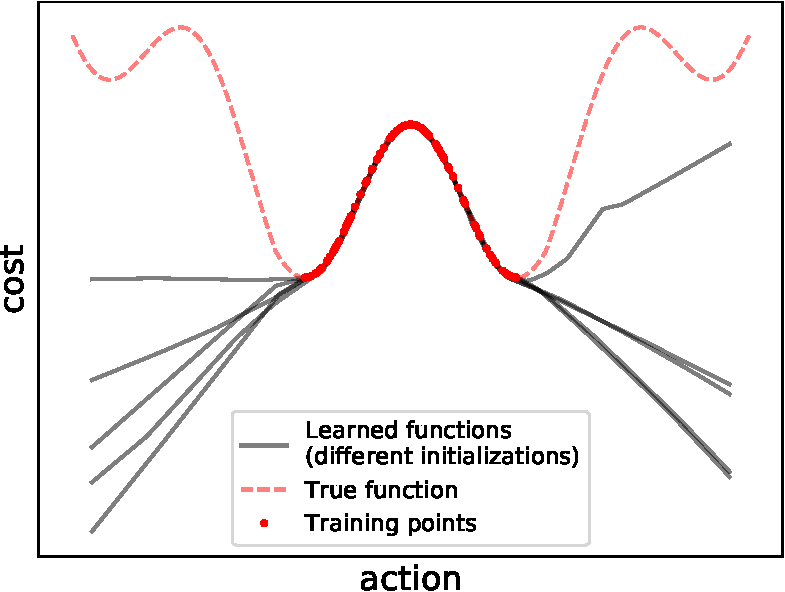
\includegraphics[width=0.3\textwidth]{figures/driving/uncertainty_example2-crop.pdf}
  \caption{\label{simple-example}Different models fitted on training points which cover a limited region the function's domain. Models make arbitrary predictions outside of this region.}
\end{wrapfigure}

However, passive imitation learning can suffer from a mismatch between input states seen at training and execution time, and may need to be augmented by interacting with an expert \citep{Dagger}.
Another option is to learn a dynamics model from observational data. However, it may make arbitrary predictions outside the domain it was trained on, which may wrongly be associated with low cost (or high reward) as shown in Figure \ref{simple-example}. A planner or policy network may then exploit these errors in the dynamics model and produce actions which lead to these wrongly optimistic states.
In the interactive setting, this problem is naturally self-correcting, since states where the model predictions are wrongly optimistic will be more likely to be experienced, and thus added to the training set, which will correct the dynamics model. However, this does not solve the problem if the dataset of environment interactions which the model is trained on is fixed.






In this work, we propose an end-to-end, model-based approach for learning driving policies from purely observational data.
We first introduce a large-scale dataset of real-world driving trajectories, which we also adapt into an environment for testing learned policies and planning methods; both dataset and environment will be made public.
%To handle this, we use recent advances in stochastic video prediction to learn an action-conditional stochastic forward model which can then be used for planning.
This dataset is highly stochastic due to the unpredictable nature of human driving, and we train both deterministic and stochastic action-conditional forward models which can then be used for planning.
%To handle this, we use recent advances in stochastic video prediction to learn an action-conditional stochastic forward model which can then be used for planning.
The key element of our approach is a differentiable term in the cost function used at planning time, representing the uncertainty of the forward model about its own predictions, which is calculated using dropout.
Minimizing this term encourages a planner or policy network to choose action sequences which keep it on the data manifold which the forward model was trained on.
We show in our experiments that model-based control using this additional regularizer substantially outperforms unregularized control, as well as both standard and model-based imitation learners, and enables learning good driving policies using only observational data with no environment interaction.

\section{Dataset and Planning Environment}
\label{dataset-and-planning}

To begin with, we summarize the dataset and planning environment which we used, with full details provided in Appendix \ref{i80-dataset-prep}.
The Next Generation Simulation program's Interstate 80 (NGSIM I-80) dataset \citep{NGSIM} consists of 45 minutes of recordings from traffic cameras made of a stretch of highway.
The driver behavior is complex and includes sudden accelerations, lane changes and merges which are difficult to predict; as such the dataset has high aleatoric uncertainty.
After recording, a viewpoint transformation is applied to rectify the perspective, and vehicles are identified and tracked throughout the video.
This yields a total 5596 car trajectories, which are then split into training ($80\%$), validation ($10\%$) and testing sets ($10\%$).

\begin{figure}[t]
  \centering
  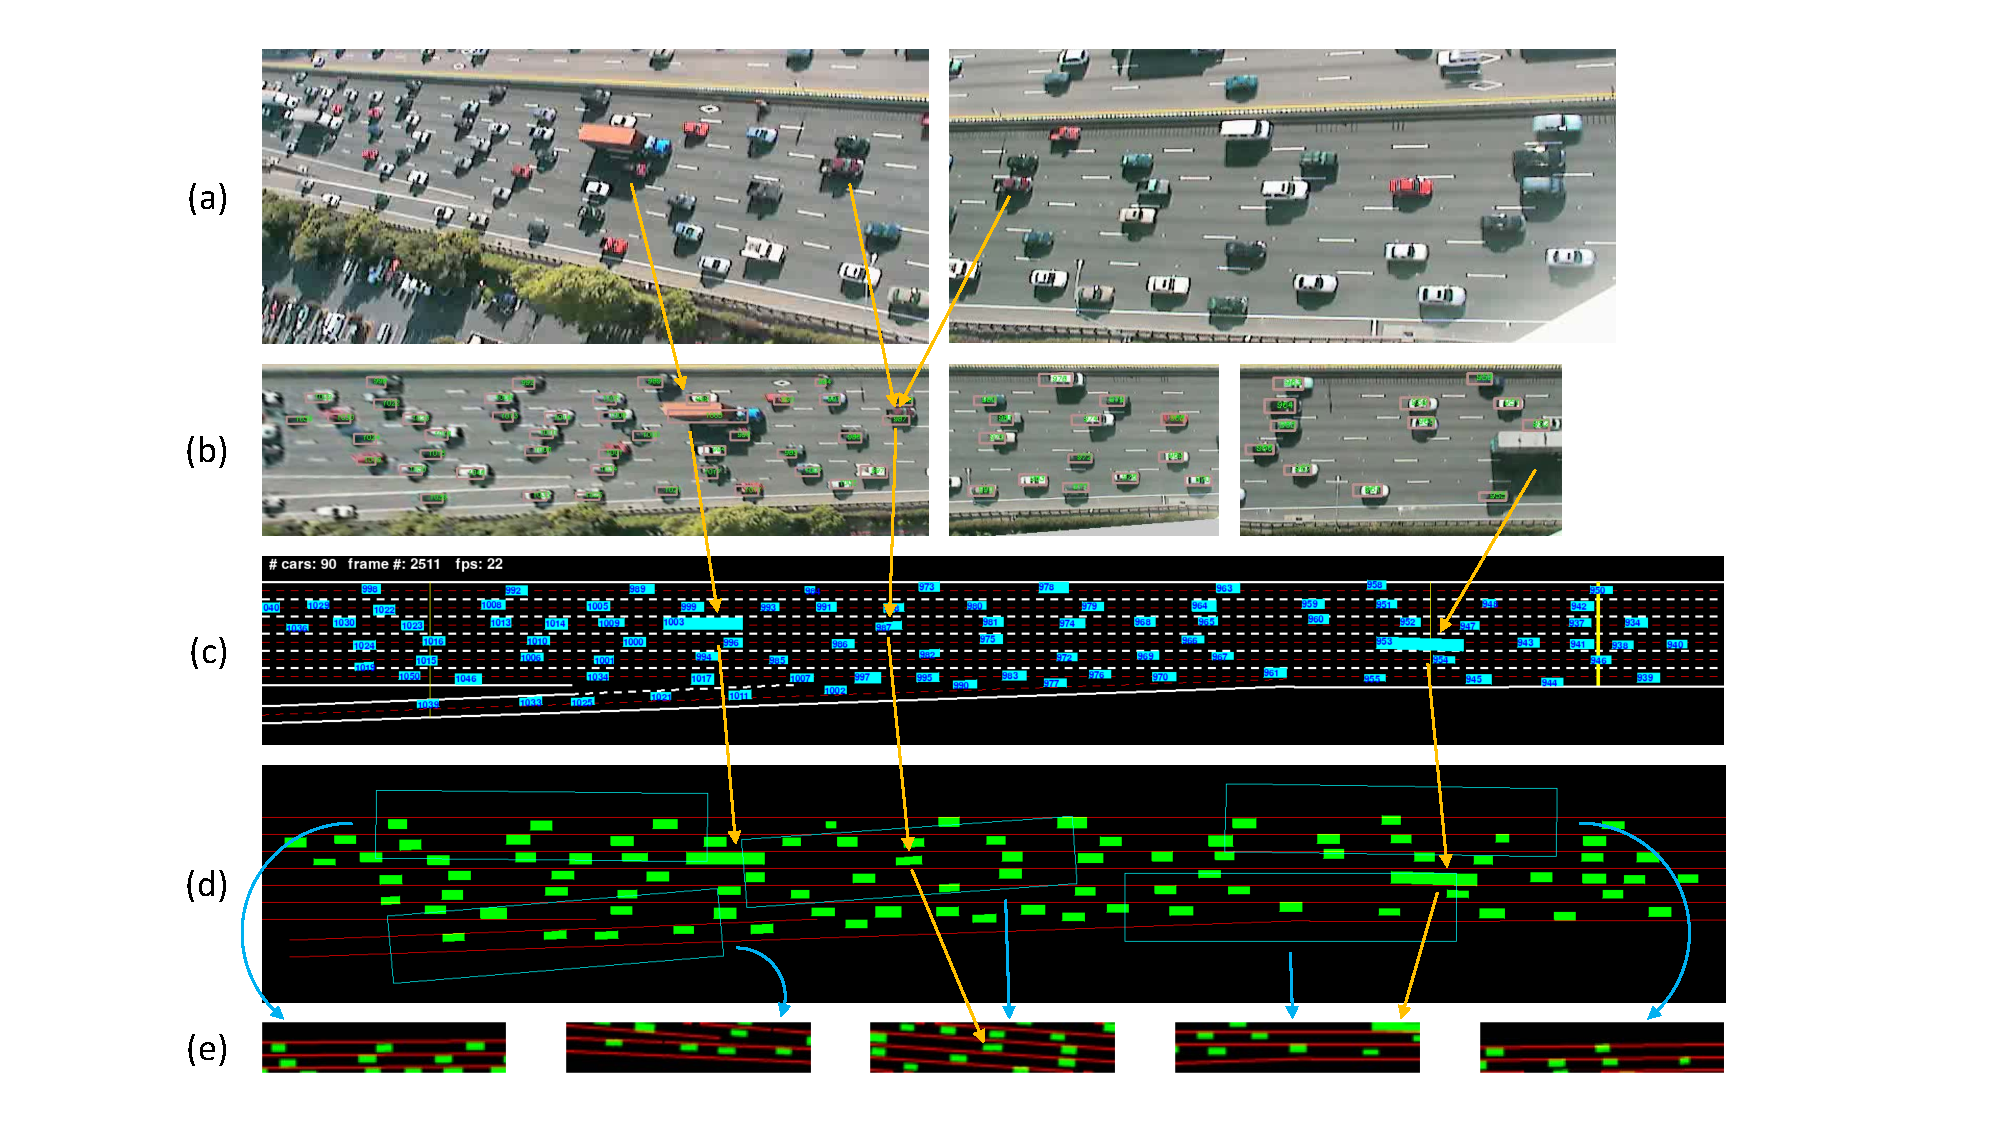
\includegraphics[width=0.8\textwidth]{figures/driving/I-80.pdf}
  \caption{
    Preprocessing pipeline for the NGSIM-I80 data set.
    Orange arrows show same vehicles across stages.
    Blue arrows show corresponding extracted context state.
    (a) Snapshots from two of the seven cameras.
    (b) View point transformation, car localisation and tracking.
    (c) Every vehicle in the simulator is initialised with starting position, initial velocity, dimensions, and ID number.
    %    A longitudinal and transverse inter-vehicle linear proximity cost is computed, which is maximum in case of collision and goes to zero if vehicles are sufficiently spaced.
    (d) Context states are extracted from rectangular regions surrounding each vehicle.
    (e) Five examples of context states extracted at the previous stage.
    Notice how vehicles oriented slightly to the left (2nd and 3rd examples) have lane markings rotated to the right.
  }
\label{I-80}
\end{figure}


We then applied additional preprocessing to obtain a state and action representations $(s_t, a_t)$ for each car, suitable for learning an action-conditional predictive model.
Our state representation $s_t$ consists of two components: an image $i_t$ representing the neighborhood of the car, and a vector $u_t$ representing its current position and velocity.
The images $i_t$ are centered around the ego car and encode both the lane emplacements and the locations of other cars.
Each image has 3 channels: the first (red) encodes the lane markings, the second (green) encodes the locations of neighboring cars, which are represented as rectangles reflecting the dimensions of each car, and the third channel (blue) represents the ego car, also scaled to the correct dimensions.
This is summarized in Figure \ref{I-80}.
We also define two cost functions to be minimized at planning time: a proximity cost which reflects how close the ego car is to neighboring cars, and a lane cost which reflects how much the ego car overlaps with lane markings. These are represented as a cost vector at each timestep, $c_t = (C_{proximity}(s_t), C_{lane}(s_t))$.
%Both costs are computed using masks in pixel space, which are pointwise multiplied with the green channel for the proximity cost and the red channel for the lane cost.
%These operations are differentiable so that we can backpropagate gradients of both costs with respect to actions through images predicted by a forward model.


We also adapted this dataset to be used as an environment to evaluate learned policies, with the same interface as OpenAI Gym \citep{OpenAIBaselines}.
Choosing a policy for neighboring cars is challenging due to a cold-start problem: to accurately evaluate a learned policy, the other cars would need to follow human-like policies which would realistically react to the controlled car, which are not available.
We take the approach of letting all the other cars in the environment follow their trajectories from the dataset, while a single car is controlled by the policy we seek to evaluate.
This approach avoids hand-designing a policy for the neighboring cars which would likely not reflect the diverse nature of human driving.
The limitation is that the neighboring cars do not react to the controlled car, which makes the problem more difficult.


\section{Planning Approach}

Our approach consists of two steps: learning an action-conditional dynamics model and cost predictor using the collected observational data, and then using this model to train a fast, feedforward policy network. We describe the two steps below.

\subsection{Action-conditional Forward Model}

We trained both deterministic and stochastic dynamics models.
Our deterministic model $f_\theta(s_{1:t}, a_t)$ takes as input a sequence of past states $s_{1:t}$ and an action $a_t$, and produces a prediction of the next state $\tilde{s}_{t+1} = (\tilde{i}_t, \tilde{u}_t)$.  
The per-sample loss which it minimizes is given by:

\begin{align}
  \label{eq:update-eqn}
  \ell(s_{1:t}, \tilde{s}_{t+1}) = \|\tilde{i}_t - i_t \|_2^2 + \| \tilde{u}_t - u_t \|_2^2
\end{align}


For the stochastic model, we adapted recent approaches for stochastic video prediction \citep{Babaeizadeh2018, Denton2018} based on Variational Autoencoders \citep{VAE}.
In addition to $s_{1:t}$ and $a_t$, the model takes as input a latent variable $z_t$ which represents the information about the next state $s_{t+1}$ which is not a deterministic function of the input.
During training, latent variables are sampled from a posterior network $q_\phi(s_{1:t}, s_{t+1})$ which outputs the parameters $(\mu_\phi, \sigma_\phi)$ of a diagonal Gaussian distribution over latent variables conditioned on the past inputs and true targets. This network is trained jointly with the prediction model using the reparameterization trick, and a term is included in the loss to minimize the KL divergence between the posterior distribution and a fixed prior $p(z)$, which in our case is an isotropic Gaussian.
Specifically, the updates are given by:

\begin{alignat}{2}
  \label{eq:update-eqn}
  &(\mu_\phi, \sigma_\phi) &&= q_\phi(s_{1:t}, s_{t+1}) \\
  &\epsilon &&\sim \mathcal{N}(0, I) \\
  &z_t &&= \mu_\phi + \sigma_\phi \cdot \epsilon \\
  &\tilde{s}_{t+1} = (\tilde{i}_{t+1}, \tilde{u}_{t+1}) &&= f_\theta(s_{1:t}, a_t, z_t)
%  &\ell(f_\theta(s_{1:t}, a_t, z_t), s_{t+1}) + \beta D_{\mbox{KL}}(f_\phi(s_{1:t}, s_{t+1}), \mathcal{N}(0, I))
\end{alignat}

The per-sample loss is given by:

\begin{align}
  \label{eq:update-eqn}
  \ell(s_{1:t}, s_{t+1}) = \|\tilde{i}_t - i_t \|_2^2 + \| \tilde{u}_t - u_t \|_2^2 + \beta D_{KL}(\mathcal{N}(\mu_\phi, \sigma_\phi) || p(z))
\end{align}

After the dynamics model is trained, we train another network $f_c$ which takes as input a state predicted by the forward model and produces an estimate of the associated proximity and lane costs. This is trained by minimizing the per sample loss:

\begin{align}
  \|f_c(f_\theta(s_{1:t}, a_t, z_t)) - c_t \|_2
\end{align}

After training, different future predictions and associated costs for a given sequence of frames can be generated by sampling different latent variables from the prior distribution.
The deterministic and stochastic models have an identical architecture except for the latent variables in the stochastic model.
Details of the prediction model and inference network architectures are given in Appendix \ref{model-details}.

\subsection{Training a Policy Network}


\begin{figure*}[t!]
    \centering
    \subfigure{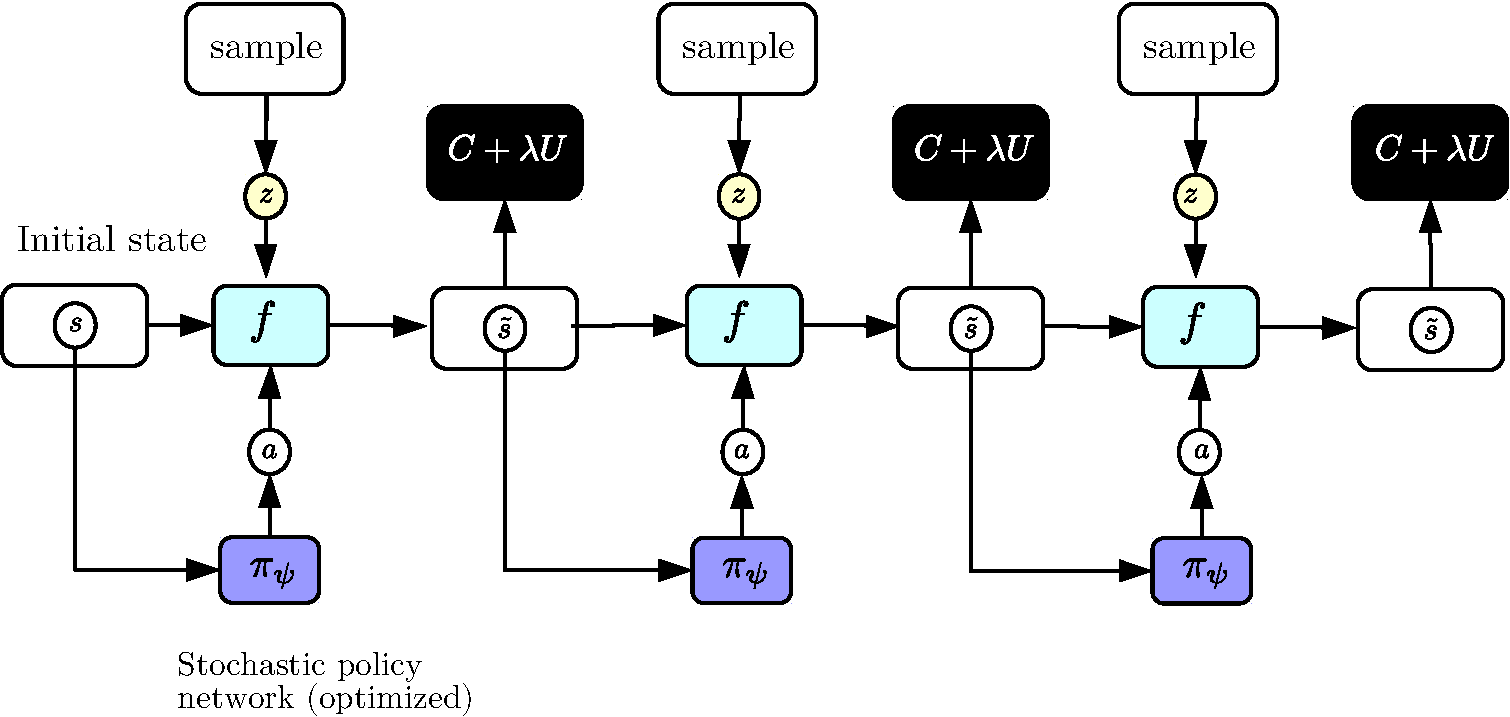
\includegraphics[width=0.7\textwidth]{figures/driving/svg-crop.pdf}} \\
    \label{svg}
    \caption{Training the policy network using the stochastic forward model. Gradients with respect to costs associated with predicted states are passed through the unrolled forward model into a policy network.}
\end{figure*}


Once the forward model and cost predictor are trained, we can use them to train a parameterized policy network $\pi_\psi$.
In the case of the deterministic forward model, we first sample an initial state sequence $s_{1:t}$ from the training set, unroll the forward model over $T$ time steps, and backpropagate gradients of the predicted costs with respect to the parameters of the policy network.
In the case of the stochastic forward model, we additionally sample latent variables from the prior for each step and input them into the forward model.
%We do this by first randomly sampling an initial input state $s_t$ from the training set, and then unrolling the forward model for $T$ steps, at each step sampling a latent variable from the prior distribution $p(z)$ and an action from the policy network using the previous state as input.
%This produces a sequence of predicted states which are passed through the cost function.
%We then backpropagate gradients of these costs through the unrolled forward model to the actions produced by the policy network, whose weights are then updated to produce actions which would lower the predicted cost.
During this process the weights of the forward model are fixed, and only the weights of the policy network are optimized. This is illustrated in Figure \ref{svg}.

    For the deterministic model, our approach is similar to that of \citep{Nguyen1989}.
    For the stochastic model, our approach is related to the $\mbox{SVG}(\infty)$ algorithm introduced in \citep{SVG}, with two differences. The first is that they sample a sequence of states $s_t, ..., s_{t+T}$ from the training set (or replay buffer), and infer the corresponding sequence of latent variables $z_t, ..., z_{t+T}$ (in our setup, this can be done using the posterior network $q_\phi$), whereas we sample latent variables from the prior. We compare the two approaches and found that using inferred latent variables causes a drop in performance, which we discuss in Section \ref{experiments}.
    The second is that they consider an interactive setting where the agent collects experience from the environment which it then uses to train its dynamics model.






    \section{Differentiable Epistemic Uncertainty Cost}
    \label{uncertainty-cost}

    We propose to augment the predicted costs with an additional cost term which penalizes the uncertainty of the forward model, calculated using dropout, and use derivatives of this cost to train the policy network.
    Dropout \citep{Dropout2012, Dropout2014} consists of randomly setting hidden units in a neural network to zero with some probability, and has been shown to substantially reduce overfitting.
    The work of \citep{Gal16} showed that a neural network trained with dropout is mathematically equivalent to an approximation of a probabilistic deep Gaussian Process model, which includes uncertainty estimates.
    A key result of this is that estimates of the neural network's epistemic uncertainty for a given input can be obtained by calculating the covariance of an outputs taken over multiple dropout masks.
    More precisely, let $f_{\theta_1}, ..., f_{\theta_K}$ denote our prediction model with $K$ different dropout masks applied to it.
    Then for some set of inputs $(s_{1:t}, a_t, z_t)$, the uncertainty of the forward model is given by the covariance matrix of the outputs under the different dropout masks (up to some constants):

    \begin{align}
      \mbox{Cov} [\{ f_{\theta_k}(s_{1:t}, a_t, z_t) \}_{k=1}^K]
    \end{align}

    We note that this uncertainty estimate is the composition of differentiable functions: each of the models induced by applying a different dropout mask is differentiable, as is the covariance operator.
    Furthermore, we can summarize the covariance matrix by taking its trace (which is equal to the sum of its eigenvalues, or equivalently the sum of the variances of the outputs across each dimension), which is also a differentiable operation. This provides a scalar estimate of uncertainty $\Omega$ which is differentiable with respect to the inputs:

    \begin{align*}
      \Omega(s_{1:t}, a_t, z_t) &= \mbox{tr} \Big[ \mbox{Cov} [\{ f_{\theta_k}(s_{1:t}, a_t, z_t) \}_{k=1}^K] \Big] \\
      &= \sum_{j=1}^D \mbox{Var}(\{ f_{\theta_k}(s_{1:t}, a_t, z_t)_j \}_{k=1}^K)
    \end{align*}


    %This allows us to obtain gradients of the inputs, and specifically actions, with respect to this measure of model uncertainty, which gives us directions in action space which would make the model more certain.

\begin{figure*}[t!]
    \centering
    \subfigure{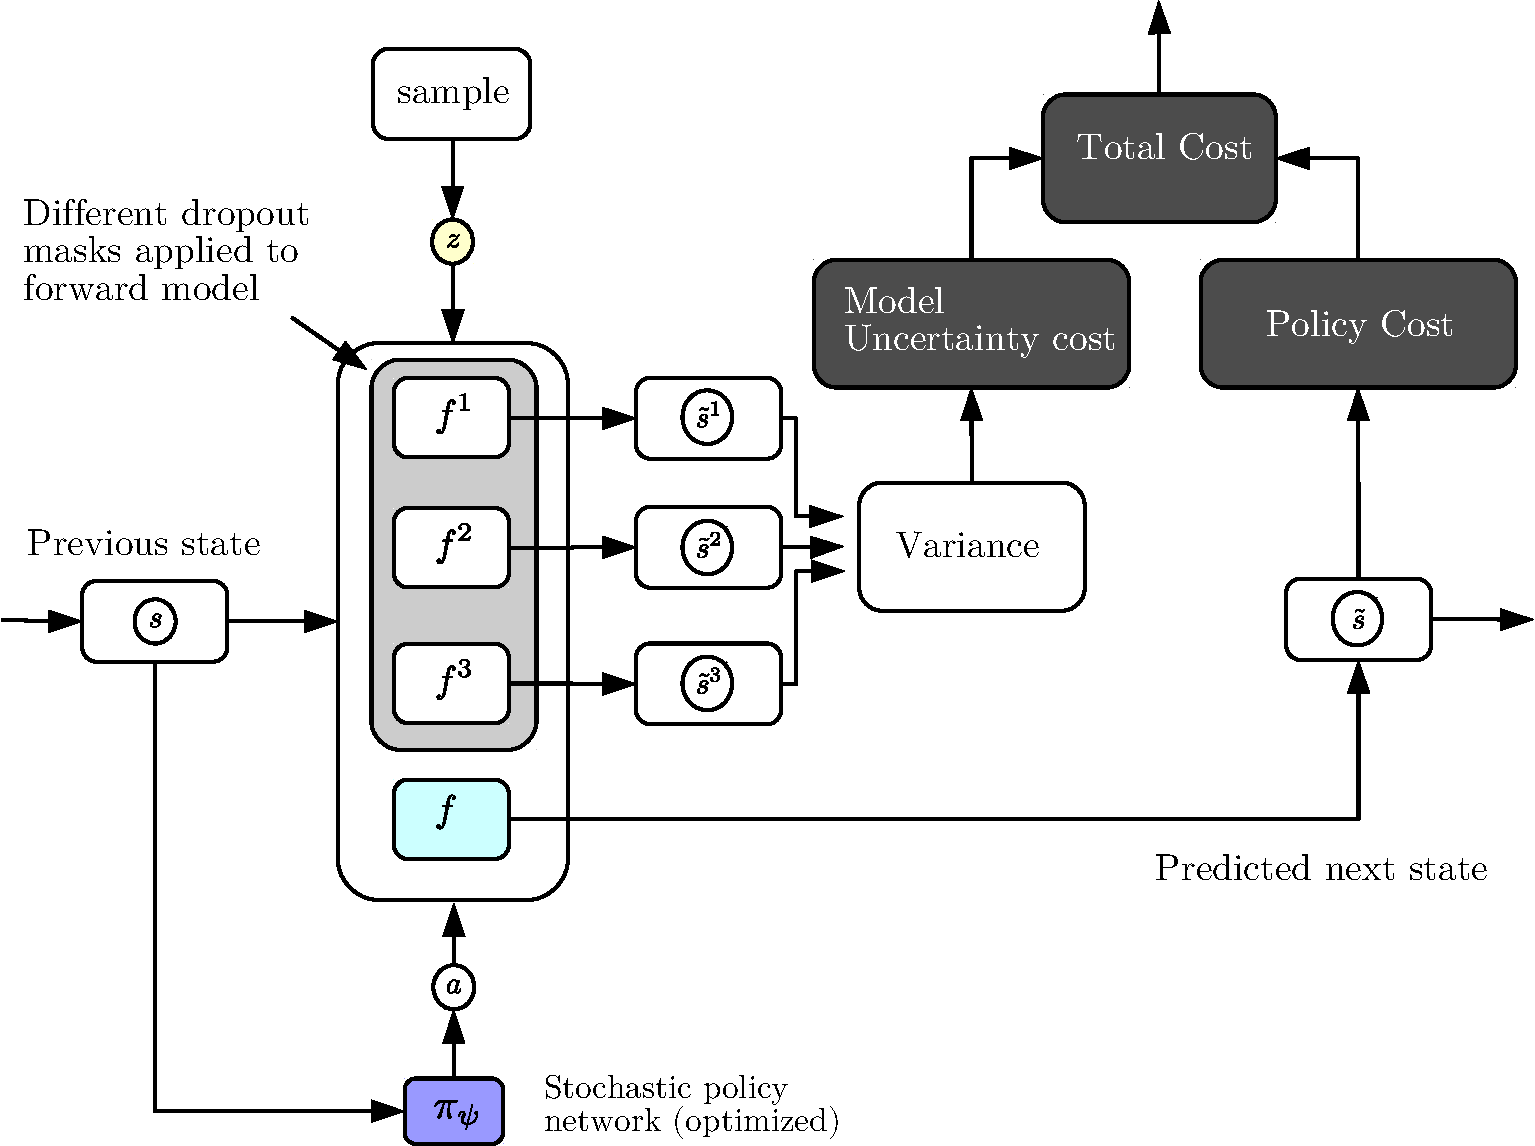
\includegraphics[width=0.8\textwidth]{figures/driving/ep_uncertainty_cost-crop.pdf}} \\
    \label{planning-methods}
    \caption{Training the policy network using the differentiable uncertainty cost, calculated using dropout.}
\end{figure*}




where $D$ is the dimensionality of the output. Minimizing this quantity with respect to actions encourages the policy network to produce actions which, when plugged into the forward model, will produce predictions which the forward model is confident about.
    To compensate for differences in baseline uncertainty across different modalities or rollout lengths, for each modality (i.e. images $i_t$ and vectors $u_t$) we estimate the empirical mean and variance of $\Omega$ for every rollout length $t$ of the forward model over the training set, to obtain $\mu_{\Omega}^t$ and $\sigma_{\Omega}^t$. We then define our epistemic uncertainty cost as follows:

    \begin{align}
      C_U(s_{1:t}, a_t, z_t) = \Big [ \frac{\Omega(s_{1:t}, a_t, z_t) - \mu_\Omega^t}{\sigma_\Omega^t} \Big]_+
    \end{align}

    If the uncertainty estimate is lower than the mean uncertainty estimate on the training set for this rollout length, this loss will be zero.
    These are cases where the model prediction is within normal uncertainty ranges. If the uncertainty estimate is higher, this loss exerts a pull to change the action so that the future state will be predicted with higher confidence by the forward model.






\section{Related Work}

In recent years, several works have explored video prediction, both in the deterministic setting \citep{VPN,Srivastava15,DentonB17} and the stochastic setting \citep{mathieu-iclr-2016, Villegas17, Babaeizadeh2018, Denton2018}.
Other works have learned action-conditional forward models which are then used for planning, starting with classic works in the 90's \citep{Nguyen1990, Schmidhuber1990, Jordan1992}, and more recently in the context of video games \citep{Oh15, Pascanu17, I2A}, robotics and continous control \citep{FinnGL16, Poke, Nagabandi2017, UPN}. Our approach to learning policies by backpropagating through a learned forward model is similar to the classic work of \citep{Nguyen1989} in the deterministic case, and the SVG framework of \citep{SVG} in the stochastic case. One difference is that both of these works use low-dimensional state representations. This allows SVG to model stochasticity using simple additive noise, whereas we use more recent stochastic models based on VAEs.

Several works have applied deep learning methods in the context of autonomous driving. The works of \citep{Pomerleau91, Bojarski16, Pan17} used neural networks to control policies trained by imitation learning, while \citep{Williams2017} learned models of the vehicle dynamics. These works focused on lane following in visually rich environments and did not focus on settings with dense traffic, which we focus on in this work. The work of \citep{Sadigh16} developed a model of the interactions between the two drivers which was then used to plan actions in simple settings, using symbolic state representations. In our work, we consider the problem of learning driving policies in dense traffic, using high-dimensional state representations which reflect the neighborhood of the ego car. %The work of \citep{Zhang16} also considered a setting with other cars, and used imitation learning together with an efficient method of querying the actions of an expert to


%Our model-based imitation learning approach is related to the work of \citep{Englert2013}, who also performed imitation learning at the level of trajectories rather than actions.
%They worked with low-dimensional state vectors representing real robots arms, which allowed them to use Gaussian Processes, and the primary source of uncertainty was measurement error. Gaussian Processes are highly data efficient, but do not scale well to high dimensions. In our setting, states include high-dimensional images and we are trying to model uncertain behavior of other drivers. The work of \citep{baram17} also used an unrolled forward model for imitation learning, but did so in the context of Generative Adversarial Imitation Learning and in deterministic environments.

%Our approach to learning policies which minimize predicted costs fits within the conceptual framework of Stochastic Value Gradients (SVG) \citep{SVG}, and extends it to a setting with high-dimensional state representations.
%This requires us to use more sophisticated stochastic models than the ones in the original work, which used additive Gaussian noise whose parameters were learned using the reparamaterization trick.
%They also considered an online setting where the agent continues to collect experience, which reduces the need for the epistemic uncertainty penalty, whereas we found this to be essential in our setting where we learn purely from observational data.

The works of \citep{DeepPilco, Chua2018} also used model uncertainty estimates calculated using dropout in the context of model-based reinforcement learning. They did so during the forward prediction step. Namely, they used different dropout masks to simulate different state trajectories which were then averaged to produce a cost estimate used to select an action.

Our model uncertainty penalty is related to the cost used in \citep{Kahn2017}, who used dropout and model ensembling to compute uncertainty estimates for a binary action-conditional collision detector for a flying drone. These estimates were then used to select actions out of a predefined set which yielded a good tradeoff between speed, predicted chance of collision and uncertainty about the prediction. In our work, we apply uncertainty estimates to the predicted states of a forward model at every time step, and backpropagate gradients through the unrolled forward model to then train a policy network by gradient descent.


The problem of covariate shift when executing a policy learned from observational data has been well-recognized in imitation learning.
It was first noted in the early work of \citep{Pomerleau91}, and was shown in \citep{Ross2010EfficientRF} to cause a regret bound which grows quadratically in the time horizon of the task.
The work of \citep{Dagger} proposed DAGGER to efficiently use expert feedback if available, which has been applied in the context of autonomous driving \citep{Zhang16}.
Our approach also addresses covariate shift, but does so without querying an expert.




\section{Experiments}
\label{experiments}

We now report experimental results. All training details can be found in Appendix \ref{training-details-appendix}.


    \subsection{Prediction Results}


    Figure \ref{prediction-results} shows predictions made by our stochastic model, as well as the deterministic model which does not use latent variables.
    The deterministic model produces predictions which become increasingly blurry further into the future, illustrating the phenomenon of averaging over different futures described in the introduction. Our stochastic model produces predictions which stay sharp far into the future.
    By sampling different sequences of latent variables, different future scenarios are generated.
    Note that the two sequences generated by the stochastic model are different from the ground truth future which occurs in the dataset.
    This is normal as the future observed in the dataset is only one of many possible ones.
    Additional video generations can be viewed at the following URL: \url{https://youtu.be/wRrQEvLq3dA}.



\begin{figure*}[t!]
    \centering
    \subfigure[Ground truth sequence]{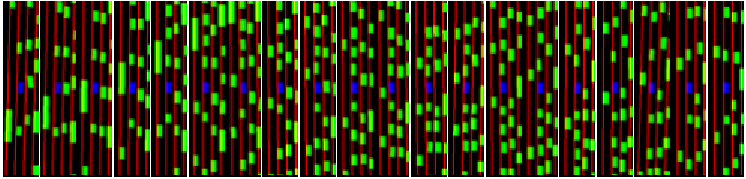
\includegraphics[width=0.48\textwidth]{figures/driving/video_predictions/truth-crop.pdf}}
    \subfigure[Deterministic Model]{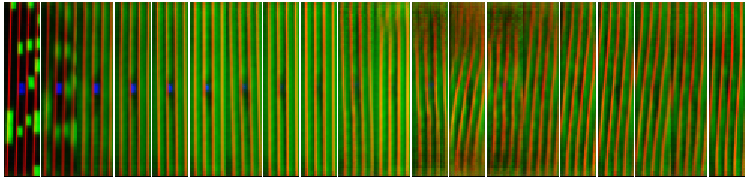
\includegraphics[width=0.48\textwidth]{figures/driving/video_predictions/det-crop.pdf}} \\
    \subfigure[Stochastic Model, sample 1]{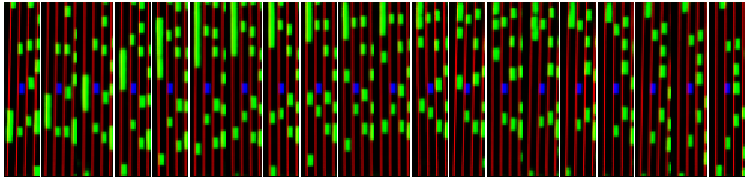
\includegraphics[width=0.48\textwidth]{figures/driving/video_predictions/pred1-crop.pdf}}
    \subfigure[Stochastic Model, sample 2]{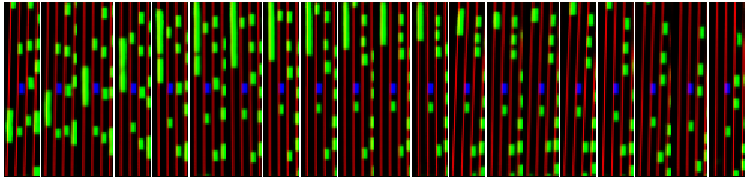
\includegraphics[width=0.48\textwidth]{figures/driving/video_predictions/pred2-crop.pdf}} \\
    \label{prediction-results}
    \caption{Video prediction results using a deterministic and stochastic model. Two different future predictions are generated by the stochastic model by sampling two different sequences of latent variables. The deterministic model averages over possible futures, producing blurred predictions.}
\end{figure*}









    \subsection{Planning Results}

    We evaluate different policies using two measures: whether the controlled car reaches the end of the road segment without colliding into another car or driving off the road, and the distance travelled before the episode ends (policies which collide quickly will travel shorter distances). All cars are initialized at the beginning of the road segment with the initial speed they were driving at in the dataset, and then are controlled by the policy being measured.

    We compared our approach against several baselines, which we briefly describe below. Full details of each of them are contained in Appendix \ref{planning-methods}.
    All policy networks have the same architecture, and all are fed the concatenation of the 20 previous states as input. They all output the parameters of a 2D diagonal Gaussian over action space, from which the next action is sampled.

    \textbf{Human:} This is the performance of the actual human trajectories observed in the testing set, which are all collision-free.

    \textbf{No action:} A simple policy which outputs an action of zero, i.e. maintains its current speed and direction.

    \textbf{Rule-Based Policy:} A hardcoded policy which outputs an action which moves the car in the opposite direction from the closest neighboring car at the current time step.

    \textbf{1-step Imitation Learner:} A policy network trained to minimize the negative log-likelihood of the true human action observed in the dataset under the parameters of its output distribution.

    \textbf{Model-Based Imitation Learner (MBIL):} An imitation learner trained to match the human trajectories in the training set, rather than the actions.
  This is done by unrolling the forward model for multiple timesteps, outputting actions by the policy network conditioned on model predictions, and minimizing the error between the final trajectory output by the forward model and the expert trajectory observed in the dataset.
  The motivation here is that if the policy network outputs an action which causes small divergence from the target trajectory at the next timestep, but large divergences later on, it will receive gradients from these larger errors backpropagated through the unrolled forward model. For the stochastic model, this requires inferring the latent variables corresponding to the training set trajectory using the posterior network $q_\phi$.





    Table \ref{main-table} compares performance for the different methods.
    The cost function which we minimize for SVG is given by:

    \begin{equation}
      C = C_{proximity} + 0.2 \cdot C_{lane} + \lambda_U \cdot C_U
    \end{equation}

    where $C_{proximity}$ and $C_{lane}$ are the proximity and lane costs described in Section \ref{dataset-and-planning}, and $C_U$ is the model uncertainty cost described in Section \ref{uncertainty-cost}. We compare results with $\lambda_U = 0$ and $\lambda_U > 0$ to show its effect.



  \begin{table}[t]
    \centering
  \begin{tabular}{|lrr|}
    \hline
    Method & Mean Distance & Success Rate (\%)  \\
    \hhline{|===|}
    Human & 1358.5 & 100.0 \\
    \hline
    No action & 566.2 & 16.2 \\
    Rule-Based Policy & - & - \\
    \hline
    A3C & - & - \\
    A3C + IL warmstart & - & - \\
    DDPG & - & - \\
    DDPG + warmstart buffer & - & - \\
    \hline
    1-step IL & 322.2 & 1.4 \\
%    MBIL (stochastic, 1 step) & 173.9 & 0.2 \\
%    MBIL (stochastic, 3 step) & 231.2 & 0.0 \\
    %    MBIL (stochastic, 5 step) & 238.6 & 0.2 \\
    MBIL (deterministic, 10 step) & - & - \\
    MBIL (deterministic, 20 step) & - & - \\
    MBIL (deterministic, 30 step) & - & - \\
    MBIL (deterministic, 40 step) & - & - \\    
    MBIL (stochastic, 10 step) & 283.7 & 0.7 \\
    MBIL (stochastic, 20 step) & 333.3 & 1.2 \\
    MBIL (stochastic, 30 step) & 348.6 & 0.7 \\
    MBIL (stochastic, 40 step) & 385.6 & 0.8 \\
    \hline
    VG-sim($\infty$) & 97.6 & 0.0 \\
    SVG-sim($\infty$) & 88.7 & 0.0 \\
    VG-sim($\infty$) + Epistemic Cost & 962.9 & 56.4 \\
%    SVG($\infty$) & 103.0 & 0.0 \\
%    SVG($\infty$) + Epistemic Cost & 525.8 & 14.5 \\
    SVG-sim($\infty$) + Epistemic Cost & \textbf{976.4} & \textbf{59.1} \\
    \hline
  \end{tabular}
  \caption{Planning performance on NGSIM dataset, measured in mean episode length. An episode ends when the controlled car collides with another car, drives off the road or reaches the end of the road segment.}
  \label{main-table}
  \end{table}


  The 1-step imitation learner performs poorly.
  Training MBIL policies with longer rollouts improves performance up to a point, but still does not beat the simple baseline of performing no action.
  Both SVG and VG without the uncertainty cost also give poor performance.
  However, adding the uncertainty cost improves performance dramatically, outperforming all other methods by a wide margin.
  Despite the difference in prediction quality observed in Figure \ref{prediction-results}, using the stochastic rather than deterministic forward model offers a relatively modest improvement in terms of the performance of the policy network it is used to train.
%  Planning with the SMPC was very computationally demanding and the results we report are only over the first 100 trajectories (out of 278) in the test set, which still took over 36 hours wallclock time.
%  In contrast, SVG with the uncertainty penalty is both fast and effective.
  Videos of the learned policies driving in the environment can be found at \url{https://youtu.be/ApjHjhyAMw0}.
  The policy learns effective behaviors such as braking, accelerating and turning to avoid other cars.


  To illustrate the effect of the epistemic uncertainty cost, we plot predictions made by the stochastic forward model for an action sequence produced by SVG policy networks trained with and without the epistemic uncertainty cost, shown in Figure \ref{svg-pred}.
  The policy network trained with the uncertainty cost produces actions which, when plugged into the forward model, yield predictions which remain on the data manifold.
  The policy network trained without the uncertainty cost, however, produces actions which produce predictions not resembling any of the training examples.
  Notice however that these predictions yield low proximity cost, since the green channel representing cars is almost zero.
  Also included in Figure \ref{svg-pred} are the average predicted proximity cost by the forward model for both policies, as well as average epistemic uncertainty cost $C_U$.
  The model trained without the uncertainty penalty produces actions for which the forward model predicts very low cost, but its uncertainty about its predictions is very high.
  The model trained with the penalty produces actions for which the forward model predicts higher cost, but with much less uncertainty.
  Including the uncertainty cost forces the policy network to produce actions which still produce reasonable predictions under the forward model, and give much better results when executed in the environment.

\begin{figure*}[t!]
    \centering
    \subfigure[with uncertainty cost]{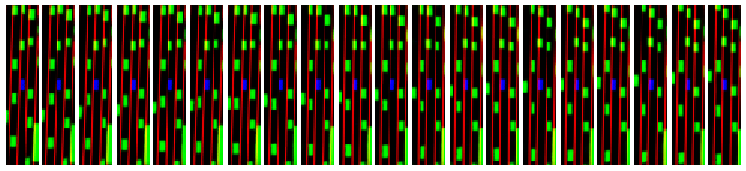
\includegraphics[width=0.48\textwidth]{figures/driving/svg_reg_prediction-crop.pdf}}
    \subfigure[without uncertainty cost]{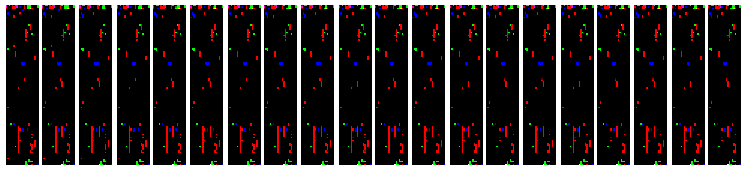
\includegraphics[width=0.48\textwidth]{figures/driving/svg_no_reg_prediction-crop.pdf}} \\
    \subfigure{

  \begin{tabular}{|lrrrr|}
    \hline
    Method & Mean Distance & Success Rate & Total Predicted Cost & $C_U$ \\
    \hhline{|=====|}
    SVG($\infty$) & 88.7 & 0.0 & 0.03 & 4087.4 \\
    SVG($\infty$) + Epistemic Cost & 976.4 & 59.1 & 0.22 & 1.1 \\
    \hline
  \end{tabular}
    }
%  Executing these actions in the environment gives very poor performance, as shown in Table \ref{main-table}.
    \caption{Predictions made by the same forward model for an action sequence produced by a policy trained \textit{with} (top) and \textit{without} (bottom) the epistemic uncertainty cost. Without the uncertainty cost, the policy network learns to output pathological action sequences which produce invalid predictions which nevertheless have low cost.}
    \label{svg-pred}
\end{figure*}

There is a significant difference in performance between $\mbox{SVG}(\infty)$ and $\mbox{SVG-sim}(\infty)$.
The main difference between these two methods is that $\mbox{SVG}(\infty)$ uses latent variables which are inferred from true trajectories in the training set using the posterior network, whereas $\mbox{SVG-sim}(\infty)$ uses latent variables which are sampled from the prior distribution $p(z)$. To better understand the effect of these two approaches, we compared the predictions made by the forward model using inferred and sampled latent variables for different sequences of actions sampled from the training set. Examples are shown in Figure \ref{action-sensitivity}. The predicted sequences using the inferred latent variables resemble the ground truth sequence, even when changing the sequence of actions input to the forward model. In contrast, when using latent variables sampled from the prior, changing the action sequence results in different sequences being predicted by the forward model.
This suggests that using inferred latent variables reduces the sensitivity of the forward model to the actions.
To quantify this, we measured the magnitude of the partial derivatives of the output images with respect to actions, averaged over the training set, and found that these derivative were much smaller when the latent variables were inferred rather than sampled.

\begin{figure*}[t!]
    \centering
  \begin{tabular}{|ccc|}
    \hline
    Method & $\| \partial i_{t+1} / \partial a_t \|_2$ & $\| \partial u_{t+1} / \partial {a_t} \|_2$\\
    \hhline{|===|}
    SVG($\infty$) & - & - \\
    SVG($\infty$) & - & - \\
    \hline
  \end{tabular}
\end{figure*}




One explanation is that the forward model encodes some factors of variation of the output due to the actions in its latent variables.
The sequence latent variables sampled from the prior are independent, which may cause these effects to cancel each other over the sequence. However, the sequence of inferred latent variables are highly dependent, and together they may explain away the effects of the actions.
%We ran an additional experiment where we trained a forward model which samples the latent variables from the prior, rather than the posterior, with probability $0.5$, in an effort to encourage it to extract more information from the actions.

%  We additionally performed several ablation experiments to understand the effects of different modeling choices, shown in table \ref{ablation}.
%  Using the action buffer has a non-negligible effect on the SMPC planning, as we see a performance drop when starting from newly initialized actions every time planning is required rather than initializing with a previously optimized action sequence.
%  It is possible that with larger numbers of gradient steps this difference in performance would decrease, but the current setup is already very expensive.
%  We also compared our TEN model to a VAE model with the same architecture and hyperparameters, except for the $\beta$ hyperparameter representing the weight of the KL term in the loss, which we set to $10^{-6}$ (we optimized over the range $\{ 1, 10^{-1},..., 10^{-6} \}$ and found that values higher than $10^{-5}$ produced blurry predictions similar to the deterministic model.
%  Performance is very similar for both models.

%  Finally, we compare SVG performance with and without masking the $z$ variables during training.
%  Not including the masking causes a performance drop due to the forward model becoming less sensitive to the actions.


  \section{Conclusion}

  \textcolor{red}{TODO: improve}
  
  In this work we have presented an end-to-end approach for learning driving policies from observational data, which includes preparing a dataset of real-world driving trajectories, adapting it to become a planning environment, training action-conditional forward models, and using them to train policies using with a new uncertainty regularizer which addresses the domain mismatch problem.
  There are several directions for future work.
  Although we have applied it here in the context of learning driving policies, the approach is general and could be used in other domains.
  Furthermore, our current approach does not capture dependencies which are longer than 20 time steps into the future, which corresponds to 2 seconds.
  We tried two different approaches to capture longer-term dependencies: learning a value function using temporal differences (which in theory can capture arbitrary length dependencies) and unrolling for more time steps, but these did not yield any improvements and sometimes hurt performance. This requires more investigation.
%  Second, we observed that the latent variables still encoded action information, although adding the dropout on the latent variables reduced this problem.
%  Finding a more principled method would be an interesting direction for future work.
  Second, it would be interesting to optimize actions or policies to produce more complex and useful behaviors, such as changing to a specified lane while avoiding other cars.
  In the current setup, the policies are optimized only to avoid collisions and stay within lanes when possible, whereas in a real-world scenario we would want a policy which can safely navigate among traffic to different locations.



\subsubsection*{Acknowledgments}

Use unnumbered third level headings for the acknowledgments. All
acknowledgments, including those to funding agencies, go at the end of the paper.

\bibliography{iclr2019_conference}
\bibliographystyle{iclr2019_conference}

\appendix

\section{Dataset and Planning Environment}
\label{i80-dataset-prep}

To begin with, we describe the details and preparation of the dataset and planning environment which we used, which are summarized in Figure \ref{I-80}.
The Next Generation Simulation program's Interstate 80 (NGSIM I-80) dataset \citep{NGSIM} consists of 45 minutes of recordings made of a stretch of highway in the San Francisco Bay Area by cameras mounted on a 30-story building overlooking the highway. The recorded area includes six freeway lanes (including a high-occupancy vehicle lane) and an onramp.
The driver behavior is complex and includes sudden accelerations, lane changes and merges which are difficult to predict; as such the dataset has high aleatoric uncertainty.
There are three time segments, each of 15 minutes, taken at different times of day which capture the transition between uncongested and congested peak period conditions.
After recording, a viewpoint transformation is applied to rectify the perspective, and vehicles are identified and tracked throughout the video; additionally, their size is inferred.
This yields a total 5596 car trajectories, represented as sequences of coordinates $\{x_t, y_t\}$. We split these trajectories into training ($80\%$), validation ($10\%$) and testing sets ($10\%$).

We then applied additional preprocessing to obtain suitable representations for learning a predictive model.
Specifically, we extracted the following: i) a state representation for each car at each time step $s_t$, which encodes the necessary information to choose an action to take, ii) an action $a_t$ which represents the action of the driver, and iii) a cost $c_t$, which associates a quality measure to each state. We describe each of these below.


\textbf{State representation}:
Our state representation consists of two components: an image representing the neighborhood of the car, and a vector representing its current position and velocity.
For the images, we rendered images centered around each car which encoded both the lane emplacements and the locations of other cars.
Each image has 3 channels: the first (red) encodes the lane markings, the second (green) encodes the locations of neighboring cars, which are represented as rectangles reflecting the dimensions of each car, and the third channel (blue) represents the ego car, also scaled to the correct dimensions.
All images have dimensions $3 \times 117 \times 24$, and are denoted by $i_t$.
\footnote{Another possibility would have been to construct feature vectors directly containing the exact coordinates of neighboring cars, however this presents several difficulties.
First, cars can enter and exit the neighborhood, and so the feature vector representing the neighboring cars would either have to be dynamically resized or padded with placeholder values.
Second, this representation would not be permutation-invariant, and it is unclear where to place a new car entering the frame.
Third, encoding the lane information in vector form would require a parametric representation of the lanes, which is more complicated.
Using images representations naturally avoids all of these difficulties.}
Two examples are shown in Figure \ref{cost}.
We also computed vectors $u_t = (p_t, \Delta p_t)$, where $p_t = (x_t, y_t)$ is the position at time $t$ and $\Delta p_t = (x_{t+1} - x_t, y_{t+1} - y_t)$ is the velocity.


\begin{figure}
  \centering
  \subfigure[19.8 km/h]{
  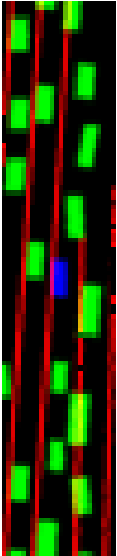
\includegraphics[height=0.3\textheight]{figures/driving/image_198-crop.pdf}
  
\includegraphics[height=0.3\textheight]{figures/driving/mask_198-crop.pdf}
  }
  \hspace{15mm}
  \subfigure[50.3 km/h]{
  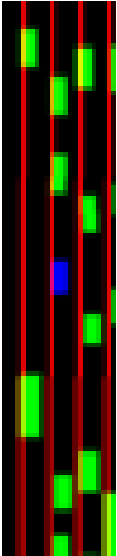
\includegraphics[height=0.3\textheight]{figures/driving/image_503-crop.pdf}
  
\includegraphics[height=0.3\textheight]{figures/driving/mask_503-crop.pdf}
  }
  \caption{Image state representations and proximity cost masks for cars going at different speeds. The higher the speed, the longer the safety distance required to maintain low cost.}
\label{cost}
\end{figure}







%Every vehicle in the simulator is initialised with starting position $\bm{p} = (x, y)$, initial velocity $v \bm{d}$ (where $v$ represents the speed and $\bm{d}$ the direction versor), correct dimensions, and identification (ID) number.
%At every time step $\Delta t = 0.1\,\text{s}$, we use the tracked trajectories (previously smoothed with a $1.5\,\text{s}$ running average) and a simplified kinematic model of a car to compute the agent actions $(a, b)$, corresponding to acceleration and tangential deviation.
%Therefore, the vehicle internal state is updated with: $\bm{p} \gets \bm{p} + v \bm{d} \Delta t$, $v \gets v + a \Delta t$, $\bm{d} \gets \bm{d} + v b \bm{d}_\perp \Delta t$, and $\bm{d} \gets \bm{d} / \lVert \bm{d} \rVert$.
%A longitudinal and transverse inter-vehicle linear proximity cost is computed, which is maximum in case of collision and goes to zero if vehicles are sufficiently spaced.
%Finally, the vehicles are drawn onto the screen canvas and displayed with their corresponding ID number.
%\textbf{(d)} Lanes and vehicles are also drawn on a secondary canvas, from which the context states are extracted.
%Rectangular regions around each vehicle --- oriented according to $\bm{d}$, of length corresponding to twice the space travelled in $1\,\text{s}$ at $130\,\text{km/h}$, of width equal four times the lane width --- scaled by a $0.5$ factor constitute the context states.
%    At this stage, the lane-crossing cost is computed using a modified morphological distance transform between each vehicle and the lane channel.



\textbf{Action representation}: Each action vector $a_t$ consists of two components: an acceleration (which can be positive or negative) which reflects the change in speed, and a change in angle.
The acceleration at a given time step is computed by taking the difference between two consecutive speeds, while the change in angle is computed by projecting the change in speed along its orthogonal direction:

\begin{align*}
  \Delta \mbox{speed} &= \| \Delta p_{t+1} \|_2 - \| \Delta p_t \|_2 \\
  \Delta \mbox{angle} &= (\Delta p_{t+1} - \Delta p_t)^\top (\Delta p_t)_\perp / \| \Delta p_t \|_2  \\
  a_t &= (\Delta \mbox{speed}, \Delta \mbox{angle}) \\
\end{align*}




\textbf{Cost}: Our cost function has two terms: a proximity cost and a lane cost. The proximity cost reflects how close the ego car is to neighboring cars, and is computed using a mask in pixel space whose width is equal to the width of a lane and whose height depends on the speed of the car. Two examples are shown in Figure \ref{cost}.
This mask is pointwise multiplied with the green channel, and the maximum value is taken to produce a scalar cost.
The lane cost uses a similar mask fixed to the size of the car, and is similarly multiplied with the red channel, thus measuring the car's overlap with the lane.
Both of these operations are differentiable so that we can backpropagate gradients with respect to these costs through images predicted by a forward model.

This preprocessing yields a set of state-action pairs $(s_t, a_t)$ (with $s_t=(i_t, u_t)$) for each car, which constitute the dataset we used for training our prediction model.
We then use the cost function to optimize action sequences at planning time, using different methods which we describe in Section \ref{planning-methods}.

We now describe how we adapted this dataset to be used as an environment to evaluate planning methods.
Building an environment for evaluating policies for autonomous driving is not obvious as it suffers from a cold-start problem.
Precisely measuring the performance of a given driving policy would require it to be evaluated in an environment where all other cars follow policies which accurately reflect human behavior.
This involves reacting appropriately both to other cars in the environment as well as the car being controlled by the policy being evaluated.
However, constructing such an environment is not possible as it would require us to already have access to a policy which drives as humans do, which in some sense is our goal in the first place. One could hand-code a driving policy to control the other cars in the environment, however is it not clear how to do so in a way which accurately reflects the diverse and often unpredictable nature of human driving.

\begin{figure}
  \centering
  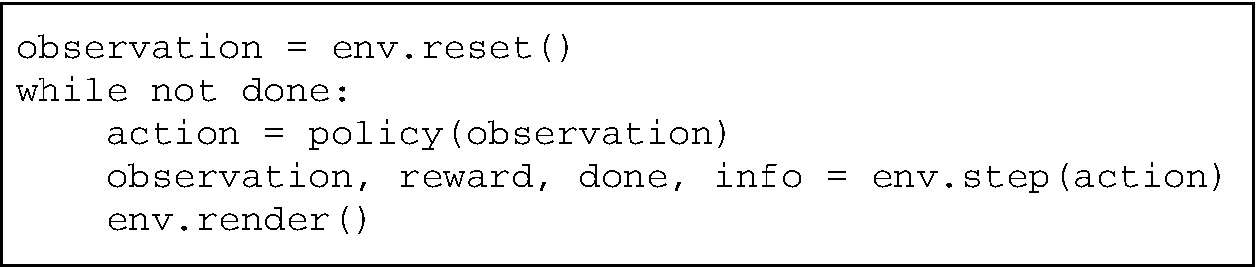
\includegraphics[width=0.8\textwidth]{figures/driving/traffic_gym_code-crop.pdf}
  \caption{NGSIM planning environment.}
\label{interface}
\end{figure}


We adopt a different approach where we let all other cars in the environment follow their trajectories in the dataset, while controlling one car with the policy we seek to evaluate.
The trajectory of the controlled car is updated as a function of the actions output by the policy, while the trajectories of the other cars remain fixed.
If the controlled car collides with another car, this is recorded and the episode ends.
This approach has the advantage that all other cars in the environment maintain behavior which is close to human-like.
The one difference with true human behavior is that the other cars do not react to the car being controlled or try to avoid it, which may cause crashes which would not occur in real life.
The driving task is thus possibly made more challenging than in a true environment, which we believe is preferable to using a hand-coded policy.
The interface is set up the same way as environments in OpenAI Gym \citep{OpenAIBaselines}, and can be accessed with a few lines of Python code, as shown in Figure \ref{interface}.



\section{Model Details}
\label{model-details}

The architecture of our forward model consists of four neural networks: a state encoder $f_\text{enc}$, an action encoder $f_\text{act}$, a decoder $f_\text{dec}$, and the posterior network $f_\phi$.
At every time step, the state encoder takes as input the concatenation of 20 previous states, each of which consists of a context image $i_t$ and a 4-dimensional vector $u_t$ encoding the car's position and velocity.
The images $i_{t-20}, ..., i_t$ are run through a 3-layer convolutional network with 64-128-256 feature maps, and the vectors $u_{t-20}, ..., u_t$ are run through a 2-layer fully connected network with 256 hidden units, whose final layers contain the same number of hidden units as the number of elements in the output of the convolutional network (we will call this number $n_H$).
The posterior network takes the same input as the encoder network, as well as the the ground truth state $s_{t+1}$, and maps them to a distribution over latent variables, from which one sample $z_t$ is drawn.
This is then passed through an expansion layer which maps it to a representation of size $n_H$.
The action encoder, which is a 2-layer fully-connected network, takes as input a 2-dimensional action $a_t$ encoding the car's acceleration and change in steering angle, and also maps it to a representation of size $n_H$.
The representations of the input states, latent variable, and action, which are all now the same size, are combined via addition.
The result is then run through a deconvolutional network with 256-128-64 feature maps, which produces a prediction for the next image $i_{t+1}$, and a 2-layer fully-connected network (with 256 hidden units) which produces a prediction for the next state vector $u_{t+1}$. These are illustrated in Figure \ref{model-components}.


\begin{figure}[t!]
    \centering
    \subfigure[$f_{enc}$]{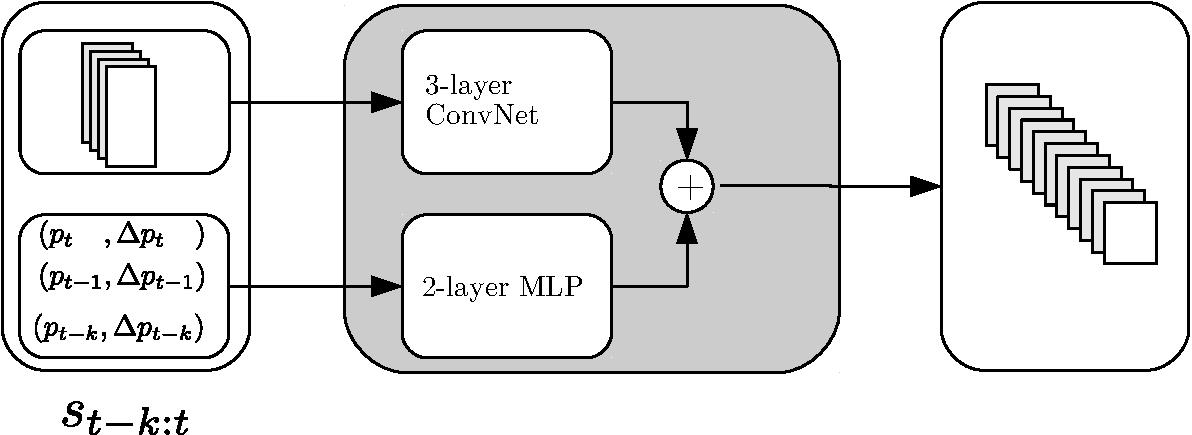
\includegraphics[width=0.45\textwidth]{figures/driving/f_enc-crop.pdf}} \\
    \subfigure[$f_{dec}$]{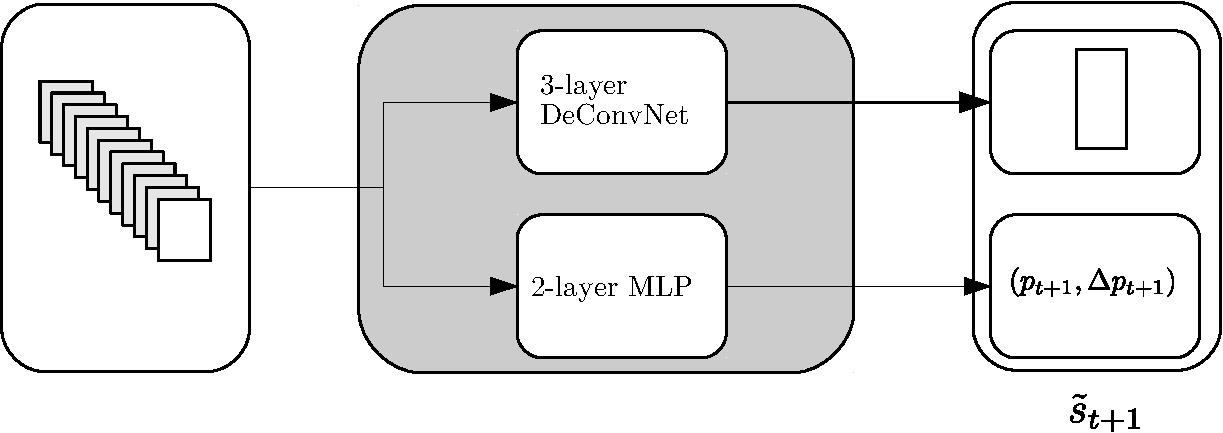
\includegraphics[width=0.45\textwidth]{figures/driving/f_dec-crop.pdf}} \\
    \subfigure[$f_\phi$]{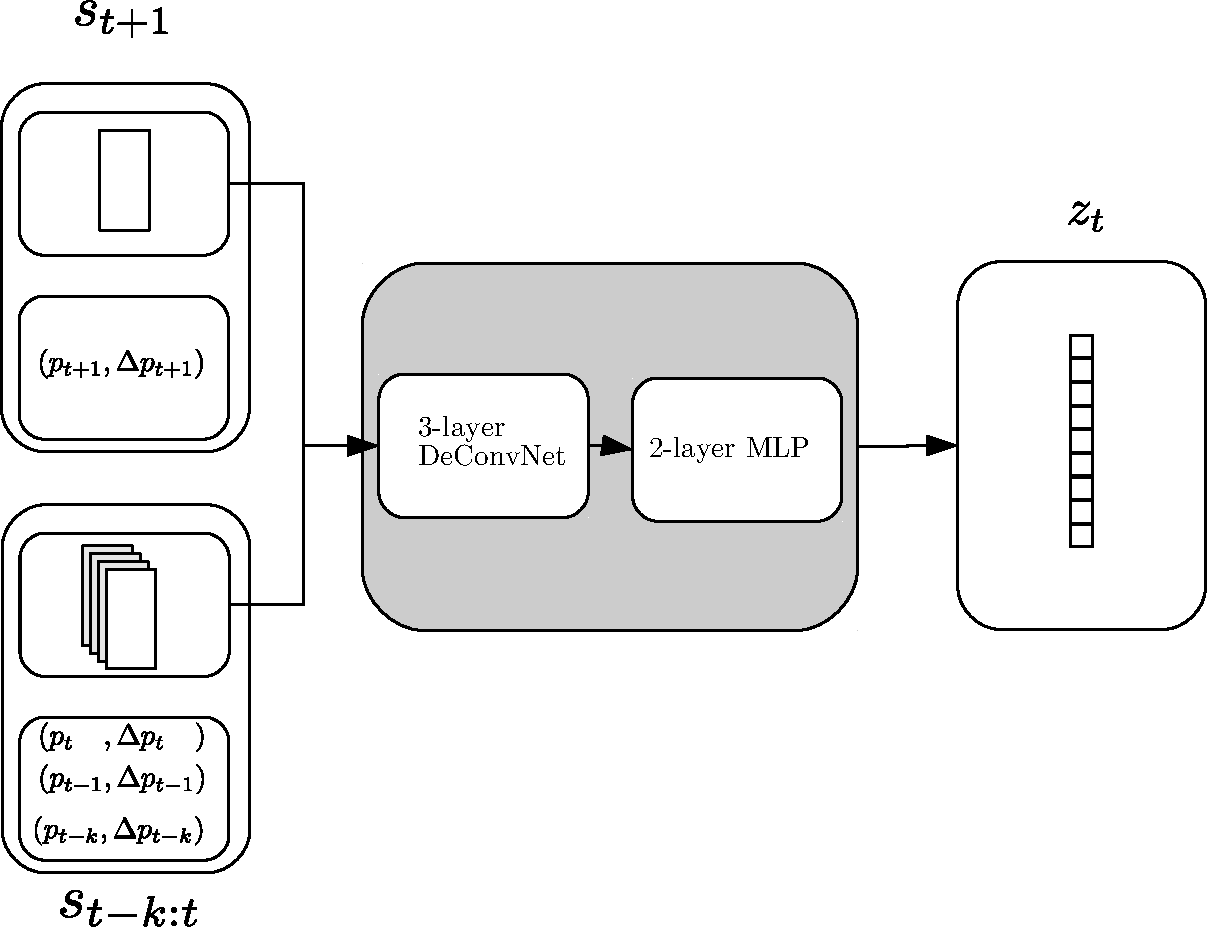
\includegraphics[width=0.45\textwidth]{figures/driving/f_phi-crop.pdf}} \\
    \caption{Individual components of the stochastic prediction model.}
\end{figure}
\label{model-components}


\section{Planning Approaches}
  \label{planning-methods}

  We now describe different planning approaches using our stochastic forward model, with diagrams shown in Figure \ref{planning-methods}.
  All methods except model-predictive control make use of a policy network which has the same architecture.
  It consists of an encoder with an identical architecture as $f_{enc}$ used in the forward model (which also takes 20 consecutive states as input), followed by a 3-layer fully connected network which outputs a 2-D mean and variance $(\mu, \sigma)$ of a diagonal Gaussian over actions.

  Two of the planning methods optimize a cost function $C$, which is a combination of the proximity and lane costs we described previously, as well as an epistemic uncertainty cost which we describe in the next section. For now, we can treat the cost as a scalar-valued differentiable function of a predicted state.


\begin{figure*}[ht!]
    \centering
    \subfigure[Stochastic Model-Based Imitation Learning (SMBIL)]{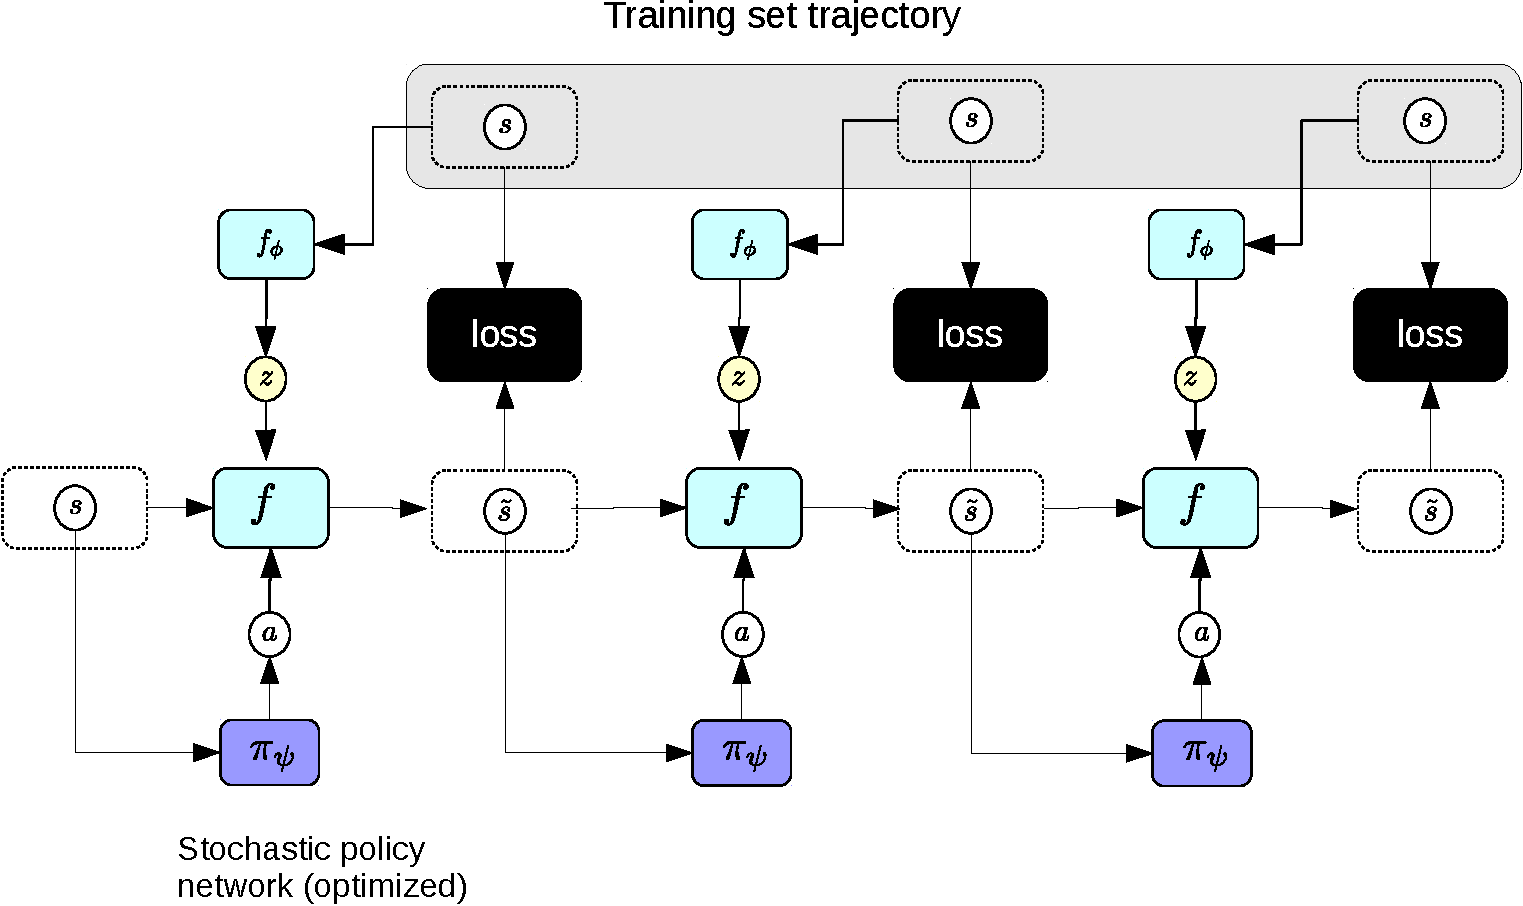
\includegraphics[width=0.5\textwidth]{figures/driving/smbil-crop.pdf}} \\
    \subfigure[Stochastic Value Gradients (SVG)]{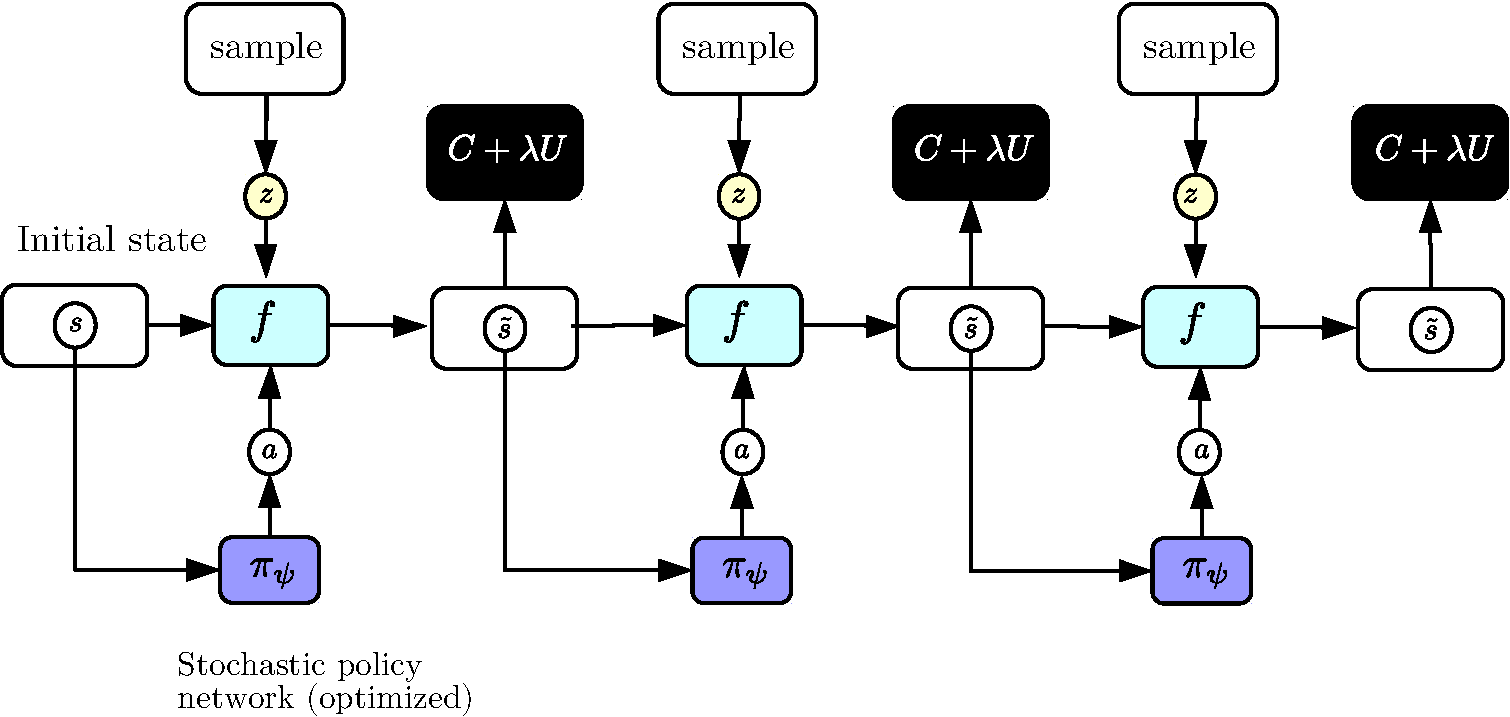
\includegraphics[width=0.5\textwidth]{figures/driving/svg-crop.pdf}} \\
    \subfigure[Stochastic Model-Predictive Control (SMPC)]{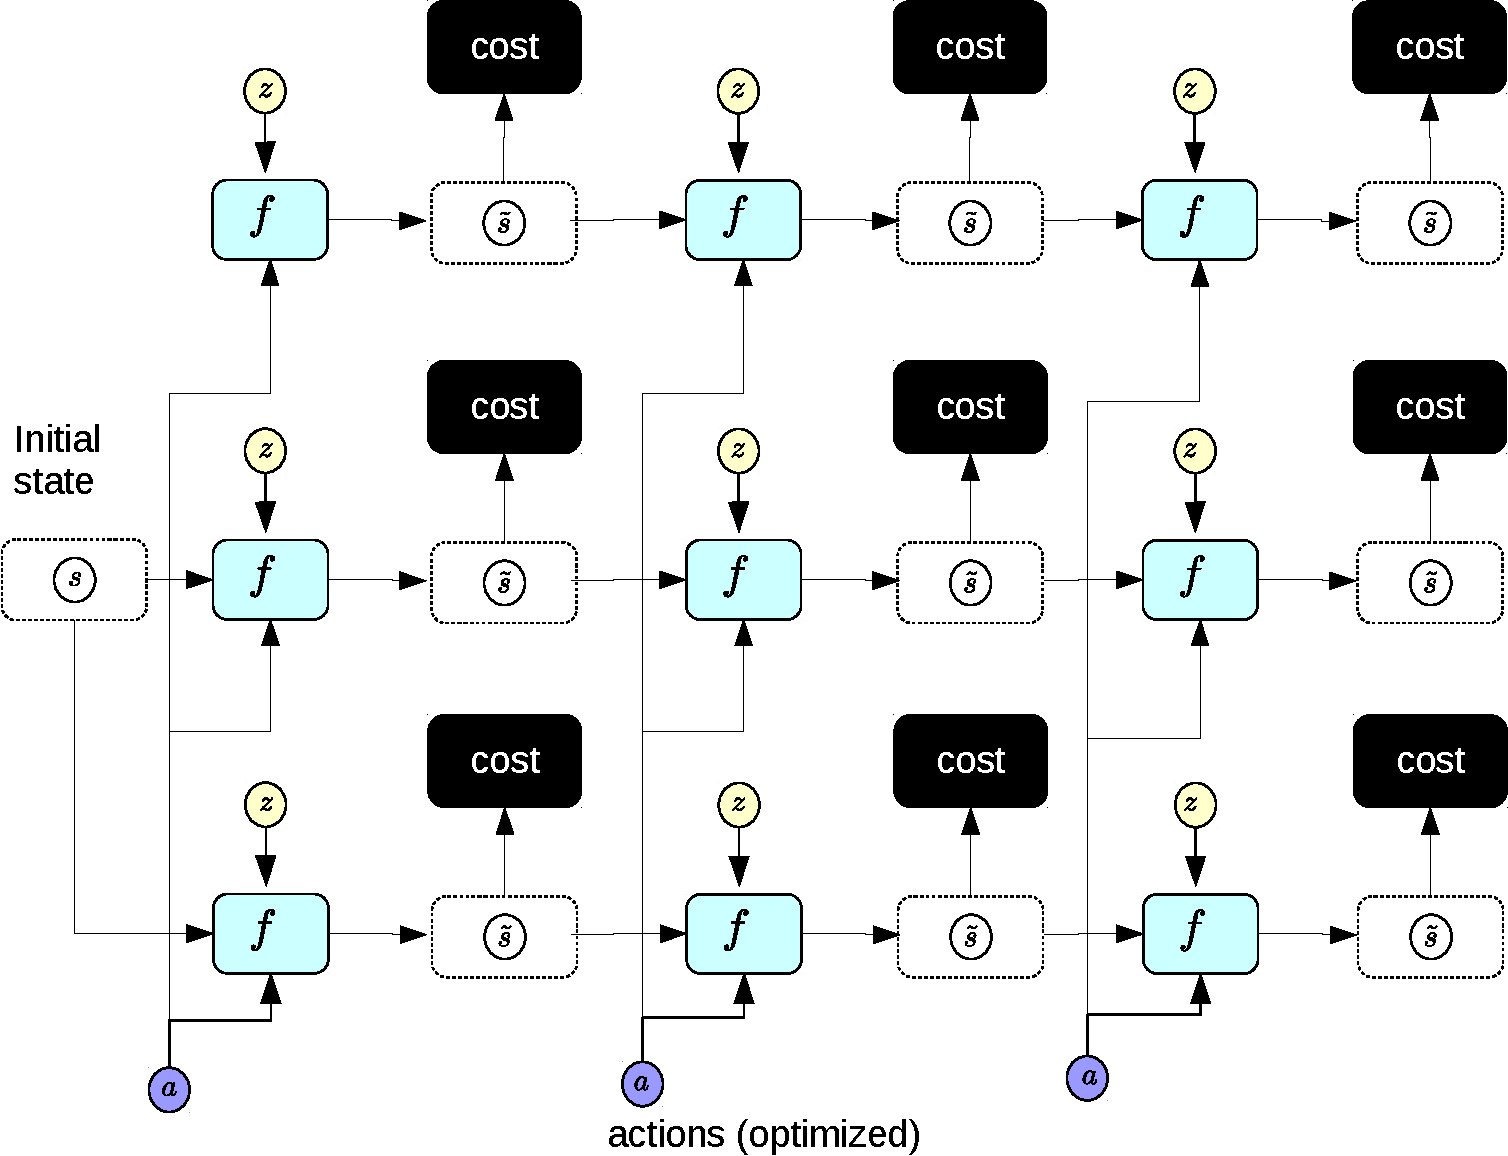
\includegraphics[width=0.5\textwidth]{figures/driving/mpc-crop.pdf}} \\
    \label{planning-methods}
    \caption{Planning Methods. SMBIL minimizes the distance between training set trajectories and trajectories predicted by the forward model under the current policy network, using latent variables inferred from the training trajectory. The other methods optimize actions or a policy network to minimize the cost predicted by the forward model, using randomly sampled sequences of latent variables.}
\end{figure*}



  \subsection{Single-Step Imitation Learning}


  The simplest approach to learning a policy from observational data is imitation learning \citep{Pomerleau91}, where a network is trained to predict expert actions from states. Here, we give the network a concatenation of 20 states $s_{1:t}$ as input and train it to minimize the negative log-likelihood of the true action observed in the dataset under the parameters of the distribution output by the model:

    \begin{align*}
    \underset{\psi}{\mbox{ argmin }} \Big[ -\mbox{ log } \mathcal{N}(a_{t+1} | \mu, \sigma) \Big],  \mbox{ such that: } (\mu, \sigma) = \pi_\psi(s_{1:t}) \\
  \end{align*}

  \subsection{Stochastic Model-Based Imitation Learning (SMBIL)}

  We also experimented with a variant of imitation learning using the learned stochastic model, which we found performed better than the standard version. One issue with imitation learning is that errors can accumulate quickly, leading to divergence from the states seen during training.
  One cause may be that the model is simply minimizing the $\ell_2$ loss in action space, which may not correspond to minimizing distances in trajectory space.
  Consider the following example where an agent is walking exactly along the side of a cliff, and must output an action which represents its angle.
  To the left is a drop, and to the right is solid ground.
  Say the expert action is to go straight, i.e. $a_{t+1} = 0$. Now consider two possible actions predicted by the network, $\tilde{a}_{t+1} = -\epsilon$ (slight left) and $\tilde{a}_{t+1} = +\epsilon$ (slight right).
  Both of these actions incur the same $\ell_2$ cost of $\epsilon$, but have very different consequences. If the agent moves slightly away from the expert action on the left side, they fall off the cliff, which causes a large deviation of their subsequent states from the expert states. If they move slightly to the right however, they stay on solid ground and their subsequent states remain close to the expert states.

  As an alternative, we experimented with training a policy to match expert \textit{trajectories}, rather than actions.
  We do this by unrolling the forward model for multiple timesteps, outputting actions by the policy network using the model predictions, and minimizing the error between the final trajectory output by the forward model and the expert trajectory observed in the dataset.
%  This is illustrated in Figure \ref{mbil-diagram}.
  The motivation here is that if the policy network outputs an action which causes small divergence from the target trajectory at the next timestep, but large divergences later on, it will receive gradients from these larger errors backpropagated through the unrolled forward model.

    \begin{align*}
    \underset{\psi}{\mbox{ argmin }} \Big[ \sum_{i=1}^{T} \ell(s_{t+i}, \tilde{s}_{t+1}) \Big],  \mbox{ such that: }
    \begin{cases}
      \tilde{s}_t = s_t \\
      z_{t+i} = f_\phi(\tilde{s}_{t+i-1}, \tilde{s}_{t+i}) \\
      \tilde{a}_{t+i} = \pi_\psi(\tilde{s}_{t+i-1}) \\
      \tilde{s}_{t+i} = f(\tilde{s}_{t+i-1}, \tilde{a}_{t+i}, z_{t+i}) \\
      \end{cases}
  \end{align*}


%  \begin{figure}[t]
%\centering
%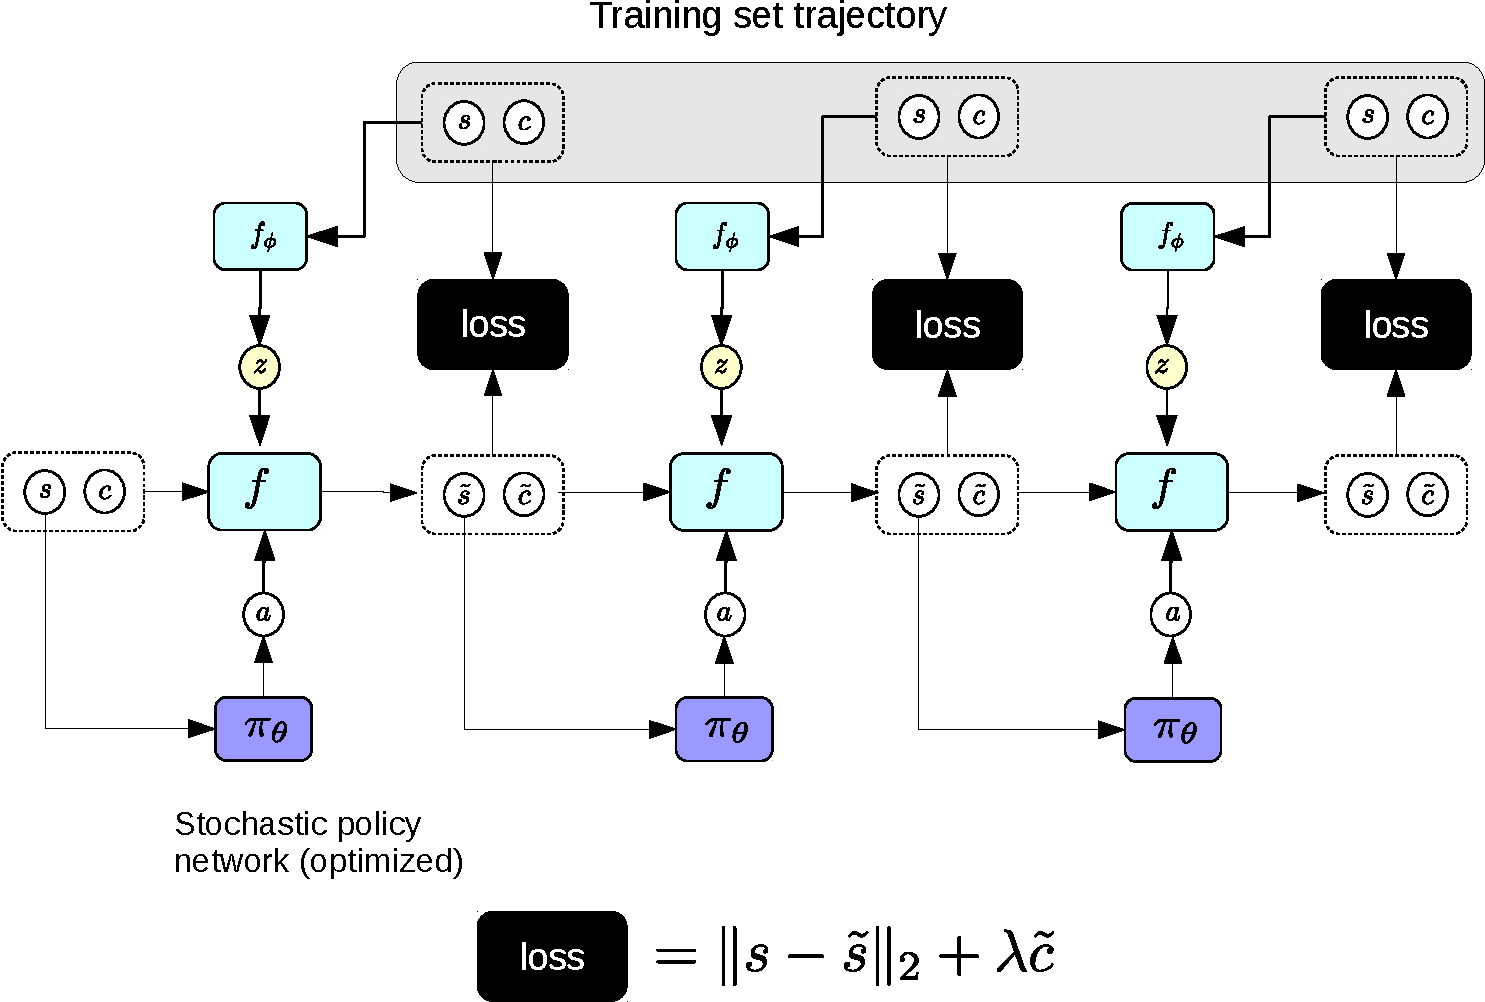
\includegraphics[width=0.95\textwidth]{figures/driving/mbil.pdf}
%\caption{Stochastic Model-Based Imitation Learning. The forward model is unrolled for several time steps and latent variables are inferred from the training sequence. Keeping these fixed, the policy network is optimized to produce actions such that the training trajectory is matched.}
%\label{mbil-diagram}
%\end{figure}


    \subsection{Stochastic Model-Predictive Control (SMPC)}
    \label{MPC}

  We also evaluated a receding-horizon model-predictive controller (MPC). At each time step, we optimize a sequence of actions over the next $T$ timesteps under the forward model and execute the first one.
  Since the model is stochastic, we sample $K$ different sequences of latent variables and optimize the same action sequence averaged over all of them.
  This requires solving the following optimization problem at each time step $t$:

  \begin{align*}
    \underset{a_t, ..., a_{t+T}}{\mbox{ argmin }} \Big[ \frac{1}{K} \sum_{k=1}^K \sum_{i=1}^{T} C(s_{t+i}^k) \Big],  \mbox{ such that: }
    \begin{cases}
      z_{t+i}^k \sim p(z) \\
      \tilde{s}_t^k = s_t  \\
      \tilde{s}_{t+i}^k = f(\tilde{s}_{t+i-1}^k, a_{t+i}, z_{t+i}^k) \\
      \end{cases}
  \end{align*}

  We solve this optimization problem by performing $N$ steps of gradient descent over the sequence of actions $a_t, ..., a_{t+T}$, during which all the sampled sequences of latent variables are held fixed.
  Intuitively, this optimization problem can be interpreted as follows. We draw $K$ different sequences of latent variables, which represent $K$ different ways in which the future can unfold.
  We then optimize a single action sequence, to minimize the predicted costs averaged over each of these possible futures.
  We thus hope to obtain an action sequence which performs well in many scenarios.

  This procedure is unfortunately expensive: it requires a total of $K \times N \times T$ model evaluations. Although the model evaluations corresponding to $K$ different futures can be done in parallel on the GPU, evaluations at different time steps and over different optimization iterations must be done sequentially.
  We found that maintaining a buffer of previously planned actions allowed us to get better performance with a relatively small number of iterations; this was proposed in \citep{Ohtsuka04}.
  Specifically, at every time step we plan for the next $T$ actions, but only execute the first even though the subsequent ones may be reasonable.
  We therefore initialize the action sequence to be optimized at the next timestep with the result of the action sequence optimized at the previous time step, shifted by one:

  \begin{equation}
    (a_t, a_{t+1}, a_{t+2}, ..., a_{T-1}, a_T) \leftarrow (a_{t+1}, a_{t+2}, ..., a_{T-1}, a_T, \mathbf{0})
  \end{equation}


  \subsection{Stochastic Value Gradients (SVG)}

  The last approach which we explored was designed to train a policy network using the learned stochastic forward model, using the framework of Stochastic Value Gradients \citep{SVG}.
  We first randomly sample an initial input state $s_t$ from the training set, sample a sequence of latent variables $z$ to represent a future scenario, and then optimize a paramaterized policy network $\pi_\psi$ to minimize the cost predicted by the forward model conditioned on this sequence of latent variables.

    \begin{align*}
    \underset{\psi}{\mbox{ argmin }} \Big[ \sum_{i=1}^{T} C(s_{t+i}) \Big],  \mbox{ such that: }
    \begin{cases}
      z_{t+i} \sim p(z) \\
      \tilde{a}_{t+i} = \pi_\psi(s_{t+i-1}) \\
      \tilde{s}_{t+i} = f(\tilde{s}_{t+i-1}, \tilde{a}_{t+i}, z_{t+i}) \\
      \end{cases}
    \end{align*}

    Our approach differs somewhat from the setup of \citep{SVG}, who used latent variables inferred from ground truth trajectories as a means to compensate for model errors. We did not find this to be a problem, possibly because we trained the forward model to make 20-step predictions, whereas they trained the forward model to make single-step predictions.



    \section{Training Details}
    \label{training-details-appendix}

    \subsection{Forward Model}
    We trained our prediction model in deterministic mode ($p=0$) for 200,000 updates, followed by another 200,000 updates in stochastic mode.
    We save the model after training in deterministic mode and treat it as a deterministic baseline.
    Our model was trained using Adam \citep{ADAM} with learning rate 0.0001 and minibatches of size 64, unrolled for 20 time steps, and with dropout ($p_{dropout}=0.1$) at every layer, which was necessary for computing the epistemic uncertainty cost during planning.

    \subsection{Policy Models}

    All policy networks have the same architecture: a 3-layer ConvNet with feature maps of size 64-128-256, followed by 3 fully-connected layers with 256 hidden units each, with the last layer outputting the parameters of a 2D Gaussian distribution over actions. All policy networks are trained with Adam with learning rate 0.0001. The SMBIL and SVG policies are trained by backpropagation through the unrolled forward model using the reparamaterization trick \citep{VAE}. The single-step imitation learner is trained to directly minimize the negative log-likelihood of the ground truth action in the dataset under the parameters output by the policy network. Both SMPC and SVG models unroll the forward model for 20 steps, and we report results for different unrolling lengths for SMBIL policies.
    The gradient descent procedure for the SMPC planner performs 5 gradient steps using Adam with learning rate 0.1. Actions are initialized to zero for the first time step, after which we used the rotating action buffer described in Section \ref{MPC}. We sampled 10 sequences of latent variables.




\end{document}
